\documentclass[11pt]{article}

    \usepackage[breakable]{tcolorbox}
    \usepackage{parskip} % Stop auto-indenting (to mimic markdown behaviour)

    \usepackage{iftex}
    \ifPDFTeX
    	\usepackage[T1]{fontenc}
    	\usepackage{mathpazo}
    \else
    	\usepackage{fontspec}
    \fi

    % Basic figure setup, for now with no caption control since it's done
    % automatically by Pandoc (which extracts ![](path) syntax from Markdown).
    \usepackage{graphicx}
    % Maintain compatibility with old templates. Remove in nbconvert 6.0
    \let\Oldincludegraphics\includegraphics
    % Ensure that by default, figures have no caption (until we provide a
    % proper Figure object with a Caption API and a way to capture that
    % in the conversion process - todo).
    \usepackage{caption}
    \DeclareCaptionFormat{nocaption}{}
    \captionsetup{format=nocaption,aboveskip=0pt,belowskip=0pt}

    \usepackage[Export]{adjustbox} % Used to constrain images to a maximum size
    \adjustboxset{max size={0.9\linewidth}{0.9\paperheight}}
    \usepackage{float}
    \floatplacement{figure}{H} % forces figures to be placed at the correct location
    \usepackage{xcolor} % Allow colors to be defined
    \usepackage{enumerate} % Needed for markdown enumerations to work
    \usepackage{geometry} % Used to adjust the document margins
    \usepackage{amsmath} % Equations
    \usepackage{amssymb} % Equations
    \usepackage{textcomp} % defines textquotesingle
    % Hack from http://tex.stackexchange.com/a/47451/13684:
    \AtBeginDocument{%
        \def\PYZsq{\textquotesingle}% Upright quotes in Pygmentized code
    }
    \usepackage{upquote} % Upright quotes for verbatim code
    \usepackage{eurosym} % defines \euro
    \usepackage[mathletters]{ucs} % Extended unicode (utf-8) support
    \usepackage{fancyvrb} % verbatim replacement that allows latex

    % The hyperref package gives us a pdf with properly built
    % internal navigation ('pdf bookmarks' for the table of contents,
    % internal cross-reference links, web links for URLs, etc.)
    \usepackage{hyperref}
    % The default LaTeX title has an obnoxious amount of whitespace. By default,
    % titling removes some of it. It also provides customization options.
    \usepackage{titling}
    \usepackage{longtable} % longtable support required by pandoc >1.10
    \usepackage{booktabs}  % table support for pandoc > 1.12.2
    \usepackage[inline]{enumitem} % IRkernel/repr support (it uses the enumerate* environment)
    \usepackage[normalem]{ulem} % ulem is needed to support strikethroughs (\sout)
                                % normalem makes italics be italics, not underlines
    \usepackage{mathrsfs}



    % Colors for the hyperref package
    \definecolor{urlcolor}{rgb}{0,.145,.698}
    \definecolor{linkcolor}{rgb}{.71,0.21,0.01}
    \definecolor{citecolor}{rgb}{.12,.54,.11}

    % ANSI colors
    \definecolor{ansi-black}{HTML}{3E424D}
    \definecolor{ansi-black-intense}{HTML}{282C36}
    \definecolor{ansi-red}{HTML}{E75C58}
    \definecolor{ansi-red-intense}{HTML}{B22B31}
    \definecolor{ansi-green}{HTML}{00A250}
    \definecolor{ansi-green-intense}{HTML}{007427}
    \definecolor{ansi-yellow}{HTML}{DDB62B}
    \definecolor{ansi-yellow-intense}{HTML}{B27D12}
    \definecolor{ansi-blue}{HTML}{208FFB}
    \definecolor{ansi-blue-intense}{HTML}{0065CA}
    \definecolor{ansi-magenta}{HTML}{D160C4}
    \definecolor{ansi-magenta-intense}{HTML}{A03196}
    \definecolor{ansi-cyan}{HTML}{60C6C8}
    \definecolor{ansi-cyan-intense}{HTML}{258F8F}
    \definecolor{ansi-white}{HTML}{C5C1B4}
    \definecolor{ansi-white-intense}{HTML}{A1A6B2}
    \definecolor{ansi-default-inverse-fg}{HTML}{FFFFFF}
    \definecolor{ansi-default-inverse-bg}{HTML}{000000}

    % commands and environments needed by pandoc snippets
    % extracted from the output of `pandoc -s`
    \providecommand{\tightlist}{%
      \setlength{\itemsep}{0pt}\setlength{\parskip}{0pt}}
    \DefineVerbatimEnvironment{Highlighting}{Verbatim}{commandchars=\\\{\}}
    % Add ',fontsize=\small' for more characters per line
    \newenvironment{Shaded}{}{}
    \newcommand{\KeywordTok}[1]{\textcolor[rgb]{0.00,0.44,0.13}{\textbf{{#1}}}}
    \newcommand{\DataTypeTok}[1]{\textcolor[rgb]{0.56,0.13,0.00}{{#1}}}
    \newcommand{\DecValTok}[1]{\textcolor[rgb]{0.25,0.63,0.44}{{#1}}}
    \newcommand{\BaseNTok}[1]{\textcolor[rgb]{0.25,0.63,0.44}{{#1}}}
    \newcommand{\FloatTok}[1]{\textcolor[rgb]{0.25,0.63,0.44}{{#1}}}
    \newcommand{\CharTok}[1]{\textcolor[rgb]{0.25,0.44,0.63}{{#1}}}
    \newcommand{\StringTok}[1]{\textcolor[rgb]{0.25,0.44,0.63}{{#1}}}
    \newcommand{\CommentTok}[1]{\textcolor[rgb]{0.38,0.63,0.69}{\textit{{#1}}}}
    \newcommand{\OtherTok}[1]{\textcolor[rgb]{0.00,0.44,0.13}{{#1}}}
    \newcommand{\AlertTok}[1]{\textcolor[rgb]{1.00,0.00,0.00}{\textbf{{#1}}}}
    \newcommand{\FunctionTok}[1]{\textcolor[rgb]{0.02,0.16,0.49}{{#1}}}
    \newcommand{\RegionMarkerTok}[1]{{#1}}
    \newcommand{\ErrorTok}[1]{\textcolor[rgb]{1.00,0.00,0.00}{\textbf{{#1}}}}
    \newcommand{\NormalTok}[1]{{#1}}

    % Additional commands for more recent versions of Pandoc
    \newcommand{\ConstantTok}[1]{\textcolor[rgb]{0.53,0.00,0.00}{{#1}}}
    \newcommand{\SpecialCharTok}[1]{\textcolor[rgb]{0.25,0.44,0.63}{{#1}}}
    \newcommand{\VerbatimStringTok}[1]{\textcolor[rgb]{0.25,0.44,0.63}{{#1}}}
    \newcommand{\SpecialStringTok}[1]{\textcolor[rgb]{0.73,0.40,0.53}{{#1}}}
    \newcommand{\ImportTok}[1]{{#1}}
    \newcommand{\DocumentationTok}[1]{\textcolor[rgb]{0.73,0.13,0.13}{\textit{{#1}}}}
    \newcommand{\AnnotationTok}[1]{\textcolor[rgb]{0.38,0.63,0.69}{\textbf{\textit{{#1}}}}}
    \newcommand{\CommentVarTok}[1]{\textcolor[rgb]{0.38,0.63,0.69}{\textbf{\textit{{#1}}}}}
    \newcommand{\VariableTok}[1]{\textcolor[rgb]{0.10,0.09,0.49}{{#1}}}
    \newcommand{\ControlFlowTok}[1]{\textcolor[rgb]{0.00,0.44,0.13}{\textbf{{#1}}}}
    \newcommand{\OperatorTok}[1]{\textcolor[rgb]{0.40,0.40,0.40}{{#1}}}
    \newcommand{\BuiltInTok}[1]{{#1}}
    \newcommand{\ExtensionTok}[1]{{#1}}
    \newcommand{\PreprocessorTok}[1]{\textcolor[rgb]{0.74,0.48,0.00}{{#1}}}
    \newcommand{\AttributeTok}[1]{\textcolor[rgb]{0.49,0.56,0.16}{{#1}}}
    \newcommand{\InformationTok}[1]{\textcolor[rgb]{0.38,0.63,0.69}{\textbf{\textit{{#1}}}}}
    \newcommand{\WarningTok}[1]{\textcolor[rgb]{0.38,0.63,0.69}{\textbf{\textit{{#1}}}}}


    % Define a nice break command that doesn't care if a line doesn't already
    % exist.
    \def\br{\hspace*{\fill} \\* }
    % Math Jax compatibility definitions
    \def\gt{>}
    \def\lt{<}
    \let\Oldtex\TeX
    \let\Oldlatex\LaTeX
    \renewcommand{\TeX}{\textrm{\Oldtex}}
    \renewcommand{\LaTeX}{\textrm{\Oldlatex}}
    % Document parameters
    % Document title
    \title{P1\_Casas\_Boston}





% Pygments definitions
\makeatletter
\def\PY@reset{\let\PY@it=\relax \let\PY@bf=\relax%
    \let\PY@ul=\relax \let\PY@tc=\relax%
    \let\PY@bc=\relax \let\PY@ff=\relax}
\def\PY@tok#1{\csname PY@tok@#1\endcsname}
\def\PY@toks#1+{\ifx\relax#1\empty\else%
    \PY@tok{#1}\expandafter\PY@toks\fi}
\def\PY@do#1{\PY@bc{\PY@tc{\PY@ul{%
    \PY@it{\PY@bf{\PY@ff{#1}}}}}}}
\def\PY#1#2{\PY@reset\PY@toks#1+\relax+\PY@do{#2}}

\expandafter\def\csname PY@tok@w\endcsname{\def\PY@tc##1{\textcolor[rgb]{0.73,0.73,0.73}{##1}}}
\expandafter\def\csname PY@tok@c\endcsname{\let\PY@it=\textit\def\PY@tc##1{\textcolor[rgb]{0.25,0.50,0.50}{##1}}}
\expandafter\def\csname PY@tok@cp\endcsname{\def\PY@tc##1{\textcolor[rgb]{0.74,0.48,0.00}{##1}}}
\expandafter\def\csname PY@tok@k\endcsname{\let\PY@bf=\textbf\def\PY@tc##1{\textcolor[rgb]{0.00,0.50,0.00}{##1}}}
\expandafter\def\csname PY@tok@kp\endcsname{\def\PY@tc##1{\textcolor[rgb]{0.00,0.50,0.00}{##1}}}
\expandafter\def\csname PY@tok@kt\endcsname{\def\PY@tc##1{\textcolor[rgb]{0.69,0.00,0.25}{##1}}}
\expandafter\def\csname PY@tok@o\endcsname{\def\PY@tc##1{\textcolor[rgb]{0.40,0.40,0.40}{##1}}}
\expandafter\def\csname PY@tok@ow\endcsname{\let\PY@bf=\textbf\def\PY@tc##1{\textcolor[rgb]{0.67,0.13,1.00}{##1}}}
\expandafter\def\csname PY@tok@nb\endcsname{\def\PY@tc##1{\textcolor[rgb]{0.00,0.50,0.00}{##1}}}
\expandafter\def\csname PY@tok@nf\endcsname{\def\PY@tc##1{\textcolor[rgb]{0.00,0.00,1.00}{##1}}}
\expandafter\def\csname PY@tok@nc\endcsname{\let\PY@bf=\textbf\def\PY@tc##1{\textcolor[rgb]{0.00,0.00,1.00}{##1}}}
\expandafter\def\csname PY@tok@nn\endcsname{\let\PY@bf=\textbf\def\PY@tc##1{\textcolor[rgb]{0.00,0.00,1.00}{##1}}}
\expandafter\def\csname PY@tok@ne\endcsname{\let\PY@bf=\textbf\def\PY@tc##1{\textcolor[rgb]{0.82,0.25,0.23}{##1}}}
\expandafter\def\csname PY@tok@nv\endcsname{\def\PY@tc##1{\textcolor[rgb]{0.10,0.09,0.49}{##1}}}
\expandafter\def\csname PY@tok@no\endcsname{\def\PY@tc##1{\textcolor[rgb]{0.53,0.00,0.00}{##1}}}
\expandafter\def\csname PY@tok@nl\endcsname{\def\PY@tc##1{\textcolor[rgb]{0.63,0.63,0.00}{##1}}}
\expandafter\def\csname PY@tok@ni\endcsname{\let\PY@bf=\textbf\def\PY@tc##1{\textcolor[rgb]{0.60,0.60,0.60}{##1}}}
\expandafter\def\csname PY@tok@na\endcsname{\def\PY@tc##1{\textcolor[rgb]{0.49,0.56,0.16}{##1}}}
\expandafter\def\csname PY@tok@nt\endcsname{\let\PY@bf=\textbf\def\PY@tc##1{\textcolor[rgb]{0.00,0.50,0.00}{##1}}}
\expandafter\def\csname PY@tok@nd\endcsname{\def\PY@tc##1{\textcolor[rgb]{0.67,0.13,1.00}{##1}}}
\expandafter\def\csname PY@tok@s\endcsname{\def\PY@tc##1{\textcolor[rgb]{0.73,0.13,0.13}{##1}}}
\expandafter\def\csname PY@tok@sd\endcsname{\let\PY@it=\textit\def\PY@tc##1{\textcolor[rgb]{0.73,0.13,0.13}{##1}}}
\expandafter\def\csname PY@tok@si\endcsname{\let\PY@bf=\textbf\def\PY@tc##1{\textcolor[rgb]{0.73,0.40,0.53}{##1}}}
\expandafter\def\csname PY@tok@se\endcsname{\let\PY@bf=\textbf\def\PY@tc##1{\textcolor[rgb]{0.73,0.40,0.13}{##1}}}
\expandafter\def\csname PY@tok@sr\endcsname{\def\PY@tc##1{\textcolor[rgb]{0.73,0.40,0.53}{##1}}}
\expandafter\def\csname PY@tok@ss\endcsname{\def\PY@tc##1{\textcolor[rgb]{0.10,0.09,0.49}{##1}}}
\expandafter\def\csname PY@tok@sx\endcsname{\def\PY@tc##1{\textcolor[rgb]{0.00,0.50,0.00}{##1}}}
\expandafter\def\csname PY@tok@m\endcsname{\def\PY@tc##1{\textcolor[rgb]{0.40,0.40,0.40}{##1}}}
\expandafter\def\csname PY@tok@gh\endcsname{\let\PY@bf=\textbf\def\PY@tc##1{\textcolor[rgb]{0.00,0.00,0.50}{##1}}}
\expandafter\def\csname PY@tok@gu\endcsname{\let\PY@bf=\textbf\def\PY@tc##1{\textcolor[rgb]{0.50,0.00,0.50}{##1}}}
\expandafter\def\csname PY@tok@gd\endcsname{\def\PY@tc##1{\textcolor[rgb]{0.63,0.00,0.00}{##1}}}
\expandafter\def\csname PY@tok@gi\endcsname{\def\PY@tc##1{\textcolor[rgb]{0.00,0.63,0.00}{##1}}}
\expandafter\def\csname PY@tok@gr\endcsname{\def\PY@tc##1{\textcolor[rgb]{1.00,0.00,0.00}{##1}}}
\expandafter\def\csname PY@tok@ge\endcsname{\let\PY@it=\textit}
\expandafter\def\csname PY@tok@gs\endcsname{\let\PY@bf=\textbf}
\expandafter\def\csname PY@tok@gp\endcsname{\let\PY@bf=\textbf\def\PY@tc##1{\textcolor[rgb]{0.00,0.00,0.50}{##1}}}
\expandafter\def\csname PY@tok@go\endcsname{\def\PY@tc##1{\textcolor[rgb]{0.53,0.53,0.53}{##1}}}
\expandafter\def\csname PY@tok@gt\endcsname{\def\PY@tc##1{\textcolor[rgb]{0.00,0.27,0.87}{##1}}}
\expandafter\def\csname PY@tok@err\endcsname{\def\PY@bc##1{\setlength{\fboxsep}{0pt}\fcolorbox[rgb]{1.00,0.00,0.00}{1,1,1}{\strut ##1}}}
\expandafter\def\csname PY@tok@kc\endcsname{\let\PY@bf=\textbf\def\PY@tc##1{\textcolor[rgb]{0.00,0.50,0.00}{##1}}}
\expandafter\def\csname PY@tok@kd\endcsname{\let\PY@bf=\textbf\def\PY@tc##1{\textcolor[rgb]{0.00,0.50,0.00}{##1}}}
\expandafter\def\csname PY@tok@kn\endcsname{\let\PY@bf=\textbf\def\PY@tc##1{\textcolor[rgb]{0.00,0.50,0.00}{##1}}}
\expandafter\def\csname PY@tok@kr\endcsname{\let\PY@bf=\textbf\def\PY@tc##1{\textcolor[rgb]{0.00,0.50,0.00}{##1}}}
\expandafter\def\csname PY@tok@bp\endcsname{\def\PY@tc##1{\textcolor[rgb]{0.00,0.50,0.00}{##1}}}
\expandafter\def\csname PY@tok@fm\endcsname{\def\PY@tc##1{\textcolor[rgb]{0.00,0.00,1.00}{##1}}}
\expandafter\def\csname PY@tok@vc\endcsname{\def\PY@tc##1{\textcolor[rgb]{0.10,0.09,0.49}{##1}}}
\expandafter\def\csname PY@tok@vg\endcsname{\def\PY@tc##1{\textcolor[rgb]{0.10,0.09,0.49}{##1}}}
\expandafter\def\csname PY@tok@vi\endcsname{\def\PY@tc##1{\textcolor[rgb]{0.10,0.09,0.49}{##1}}}
\expandafter\def\csname PY@tok@vm\endcsname{\def\PY@tc##1{\textcolor[rgb]{0.10,0.09,0.49}{##1}}}
\expandafter\def\csname PY@tok@sa\endcsname{\def\PY@tc##1{\textcolor[rgb]{0.73,0.13,0.13}{##1}}}
\expandafter\def\csname PY@tok@sb\endcsname{\def\PY@tc##1{\textcolor[rgb]{0.73,0.13,0.13}{##1}}}
\expandafter\def\csname PY@tok@sc\endcsname{\def\PY@tc##1{\textcolor[rgb]{0.73,0.13,0.13}{##1}}}
\expandafter\def\csname PY@tok@dl\endcsname{\def\PY@tc##1{\textcolor[rgb]{0.73,0.13,0.13}{##1}}}
\expandafter\def\csname PY@tok@s2\endcsname{\def\PY@tc##1{\textcolor[rgb]{0.73,0.13,0.13}{##1}}}
\expandafter\def\csname PY@tok@sh\endcsname{\def\PY@tc##1{\textcolor[rgb]{0.73,0.13,0.13}{##1}}}
\expandafter\def\csname PY@tok@s1\endcsname{\def\PY@tc##1{\textcolor[rgb]{0.73,0.13,0.13}{##1}}}
\expandafter\def\csname PY@tok@mb\endcsname{\def\PY@tc##1{\textcolor[rgb]{0.40,0.40,0.40}{##1}}}
\expandafter\def\csname PY@tok@mf\endcsname{\def\PY@tc##1{\textcolor[rgb]{0.40,0.40,0.40}{##1}}}
\expandafter\def\csname PY@tok@mh\endcsname{\def\PY@tc##1{\textcolor[rgb]{0.40,0.40,0.40}{##1}}}
\expandafter\def\csname PY@tok@mi\endcsname{\def\PY@tc##1{\textcolor[rgb]{0.40,0.40,0.40}{##1}}}
\expandafter\def\csname PY@tok@il\endcsname{\def\PY@tc##1{\textcolor[rgb]{0.40,0.40,0.40}{##1}}}
\expandafter\def\csname PY@tok@mo\endcsname{\def\PY@tc##1{\textcolor[rgb]{0.40,0.40,0.40}{##1}}}
\expandafter\def\csname PY@tok@ch\endcsname{\let\PY@it=\textit\def\PY@tc##1{\textcolor[rgb]{0.25,0.50,0.50}{##1}}}
\expandafter\def\csname PY@tok@cm\endcsname{\let\PY@it=\textit\def\PY@tc##1{\textcolor[rgb]{0.25,0.50,0.50}{##1}}}
\expandafter\def\csname PY@tok@cpf\endcsname{\let\PY@it=\textit\def\PY@tc##1{\textcolor[rgb]{0.25,0.50,0.50}{##1}}}
\expandafter\def\csname PY@tok@c1\endcsname{\let\PY@it=\textit\def\PY@tc##1{\textcolor[rgb]{0.25,0.50,0.50}{##1}}}
\expandafter\def\csname PY@tok@cs\endcsname{\let\PY@it=\textit\def\PY@tc##1{\textcolor[rgb]{0.25,0.50,0.50}{##1}}}

\def\PYZbs{\char`\\}
\def\PYZus{\char`\_}
\def\PYZob{\char`\{}
\def\PYZcb{\char`\}}
\def\PYZca{\char`\^}
\def\PYZam{\char`\&}
\def\PYZlt{\char`\<}
\def\PYZgt{\char`\>}
\def\PYZsh{\char`\#}
\def\PYZpc{\char`\%}
\def\PYZdl{\char`\$}
\def\PYZhy{\char`\-}
\def\PYZsq{\char`\'}
\def\PYZdq{\char`\"}
\def\PYZti{\char`\~}
% for compatibility with earlier versions
\def\PYZat{@}
\def\PYZlb{[}
\def\PYZrb{]}
\makeatother


    % For linebreaks inside Verbatim environment from package fancyvrb.
    \makeatletter
        \newbox\Wrappedcontinuationbox
        \newbox\Wrappedvisiblespacebox
        \newcommand*\Wrappedvisiblespace {\textcolor{red}{\textvisiblespace}}
        \newcommand*\Wrappedcontinuationsymbol {\textcolor{red}{\llap{\tiny$\m@th\hookrightarrow$}}}
        \newcommand*\Wrappedcontinuationindent {3ex }
        \newcommand*\Wrappedafterbreak {\kern\Wrappedcontinuationindent\copy\Wrappedcontinuationbox}
        % Take advantage of the already applied Pygments mark-up to insert
        % potential linebreaks for TeX processing.
        %        {, <, #, %, $, ' and ": go to next line.
        %        _, }, ^, &, >, - and ~: stay at end of broken line.
        % Use of \textquotesingle for straight quote.
        \newcommand*\Wrappedbreaksatspecials {%
            \def\PYGZus{\discretionary{\char`\_}{\Wrappedafterbreak}{\char`\_}}%
            \def\PYGZob{\discretionary{}{\Wrappedafterbreak\char`\{}{\char`\{}}%
            \def\PYGZcb{\discretionary{\char`\}}{\Wrappedafterbreak}{\char`\}}}%
            \def\PYGZca{\discretionary{\char`\^}{\Wrappedafterbreak}{\char`\^}}%
            \def\PYGZam{\discretionary{\char`\&}{\Wrappedafterbreak}{\char`\&}}%
            \def\PYGZlt{\discretionary{}{\Wrappedafterbreak\char`\<}{\char`\<}}%
            \def\PYGZgt{\discretionary{\char`\>}{\Wrappedafterbreak}{\char`\>}}%
            \def\PYGZsh{\discretionary{}{\Wrappedafterbreak\char`\#}{\char`\#}}%
            \def\PYGZpc{\discretionary{}{\Wrappedafterbreak\char`\%}{\char`\%}}%
            \def\PYGZdl{\discretionary{}{\Wrappedafterbreak\char`\$}{\char`\$}}%
            \def\PYGZhy{\discretionary{\char`\-}{\Wrappedafterbreak}{\char`\-}}%
            \def\PYGZsq{\discretionary{}{\Wrappedafterbreak\textquotesingle}{\textquotesingle}}%
            \def\PYGZdq{\discretionary{}{\Wrappedafterbreak\char`\"}{\char`\"}}%
            \def\PYGZti{\discretionary{\char`\~}{\Wrappedafterbreak}{\char`\~}}%
        }
        % Some characters . , ; ? ! / are not pygmentized.
        % This macro makes them "active" and they will insert potential linebreaks
        \newcommand*\Wrappedbreaksatpunct {%
            \lccode`\~`\.\lowercase{\def~}{\discretionary{\hbox{\char`\.}}{\Wrappedafterbreak}{\hbox{\char`\.}}}%
            \lccode`\~`\,\lowercase{\def~}{\discretionary{\hbox{\char`\,}}{\Wrappedafterbreak}{\hbox{\char`\,}}}%
            \lccode`\~`\;\lowercase{\def~}{\discretionary{\hbox{\char`\;}}{\Wrappedafterbreak}{\hbox{\char`\;}}}%
            \lccode`\~`\:\lowercase{\def~}{\discretionary{\hbox{\char`\:}}{\Wrappedafterbreak}{\hbox{\char`\:}}}%
            \lccode`\~`\?\lowercase{\def~}{\discretionary{\hbox{\char`\?}}{\Wrappedafterbreak}{\hbox{\char`\?}}}%
            \lccode`\~`\!\lowercase{\def~}{\discretionary{\hbox{\char`\!}}{\Wrappedafterbreak}{\hbox{\char`\!}}}%
            \lccode`\~`\/\lowercase{\def~}{\discretionary{\hbox{\char`\/}}{\Wrappedafterbreak}{\hbox{\char`\/}}}%
            \catcode`\.\active
            \catcode`\,\active
            \catcode`\;\active
            \catcode`\:\active
            \catcode`\?\active
            \catcode`\!\active
            \catcode`\/\active
            \lccode`\~`\~
        }
    \makeatother

    \let\OriginalVerbatim=\Verbatim
    \makeatletter
    \renewcommand{\Verbatim}[1][1]{%
        %\parskip\z@skip
        \sbox\Wrappedcontinuationbox {\Wrappedcontinuationsymbol}%
        \sbox\Wrappedvisiblespacebox {\FV@SetupFont\Wrappedvisiblespace}%
        \def\FancyVerbFormatLine ##1{\hsize\linewidth
            \vtop{\raggedright\hyphenpenalty\z@\exhyphenpenalty\z@
                \doublehyphendemerits\z@\finalhyphendemerits\z@
                \strut ##1\strut}%
        }%
        % If the linebreak is at a space, the latter will be displayed as visible
        % space at end of first line, and a continuation symbol starts next line.
        % Stretch/shrink are however usually zero for typewriter font.
        \def\FV@Space {%
            \nobreak\hskip\z@ plus\fontdimen3\font minus\fontdimen4\font
            \discretionary{\copy\Wrappedvisiblespacebox}{\Wrappedafterbreak}
            {\kern\fontdimen2\font}%
        }%

        % Allow breaks at special characters using \PYG... macros.
        \Wrappedbreaksatspecials
        % Breaks at punctuation characters . , ; ? ! and / need catcode=\active
        \OriginalVerbatim[#1,codes*=\Wrappedbreaksatpunct]%
    }
    \makeatother

    % Exact colors from NB
    \definecolor{incolor}{HTML}{303F9F}
    \definecolor{outcolor}{HTML}{D84315}
    \definecolor{cellborder}{HTML}{CFCFCF}
    \definecolor{cellbackground}{HTML}{F7F7F7}

    % prompt
    \makeatletter
    \newcommand{\boxspacing}{\kern\kvtcb@left@rule\kern\kvtcb@boxsep}
    \makeatother
    \newcommand{\prompt}[4]{
        \ttfamily\llap{{\color{#2}[#3]:\hspace{3pt}#4}}\vspace{-\baselineskip}
    }



    % Prevent overflowing lines due to hard-to-break entities
    \sloppy
    % Setup hyperref package
    \hypersetup{
      breaklinks=true,  % so long urls are correctly broken across lines
      colorlinks=true,
      urlcolor=urlcolor,
      linkcolor=linkcolor,
      citecolor=citecolor,
      }
    % Slightly bigger margins than the latex defaults

    \geometry{verbose,tmargin=1in,bmargin=1in,lmargin=1in,rmargin=1in}



\begin{document}

    \maketitle




    \hypertarget{pruxe1ctica-1-casas-en-boston}{%
\section{Práctica 1: Casas en
Boston}\label{pruxe1ctica-1-casas-en-boston}}

Esta es la primera práctica de la asignatura de \textbf{Análisis de
Datos} del grado de \emph{Ingeniería Informática} de la \emph{UC3M}
durante el curso 2020/21.

Autores:\\
\textbf{\emph{Alba Reinders Sánchez}}, 100383444, gr.83\\
\textbf{\emph{Alejandro Valverde Mahou}}, 100383383, gr.83

    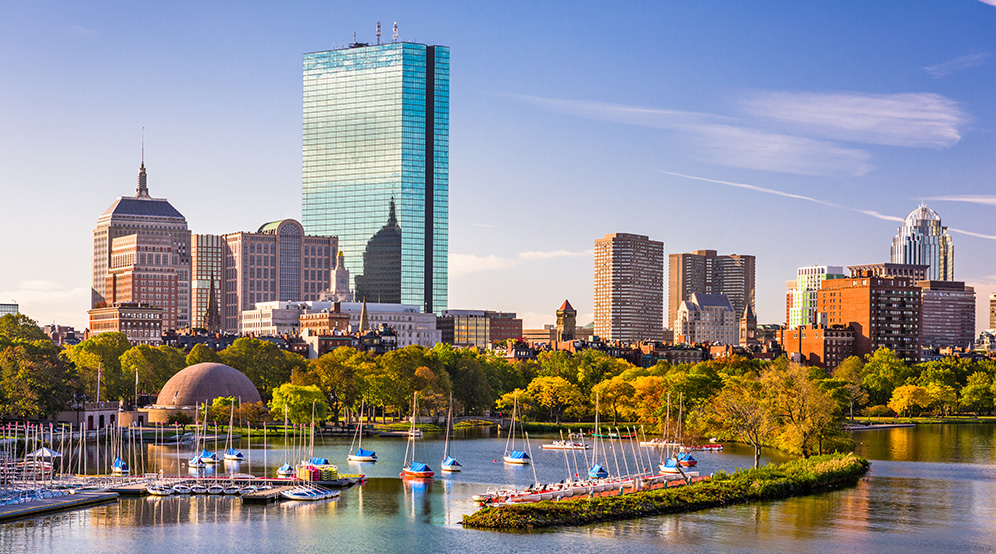
\includegraphics{./imagen_boston.jpg}

    El objetivo de esta práctica es predecir mediante un \emph{modelo de
regresión} una estimación del precio medio de la vivienda en distintas
zonas de Boston.

El conjunto de datos está compuesto por \textbf{506} ejemplos, cada uno
con \textbf{13} atributos. Más la clase a predecir.

Para ver qué representa cada uno de estos atributos, visitar el artículo
original:
\href{https://www.researchgate.net/publication/4974606_Hedonic_housing_prices_and_the_demand_for_clean_air}{Harrison
Jr, David, and Daniel L. Rubinfeld. ``Hedonichousingpricesand
thedemandforcleanair.''Journalof environmentaleconomicsand management5,
no. 1 (1978): pp.~81--102}

    \begin{tcolorbox}[breakable, size=fbox, boxrule=1pt, pad at break*=1mm,colback=cellbackground, colframe=cellborder]
\prompt{In}{incolor}{1}{\boxspacing}
\begin{Verbatim}[commandchars=\\\{\}]
\PY{c+c1}{\PYZsh{} Cabecera de los datos (atributos)}
\PY{n}{header} \PY{o}{=} \PY{p}{[}\PY{l+s+s1}{\PYZsq{}}\PY{l+s+s1}{crim}\PY{l+s+s1}{\PYZsq{}}\PY{p}{,} \PY{l+s+s1}{\PYZsq{}}\PY{l+s+s1}{zn}\PY{l+s+s1}{\PYZsq{}}\PY{p}{,} \PY{l+s+s1}{\PYZsq{}}\PY{l+s+s1}{indus}\PY{l+s+s1}{\PYZsq{}}\PY{p}{,} \PY{l+s+s1}{\PYZsq{}}\PY{l+s+s1}{chas}\PY{l+s+s1}{\PYZsq{}}\PY{p}{,} \PY{l+s+s1}{\PYZsq{}}\PY{l+s+s1}{nox}\PY{l+s+s1}{\PYZsq{}}\PY{p}{,} \PY{l+s+s1}{\PYZsq{}}\PY{l+s+s1}{rm}\PY{l+s+s1}{\PYZsq{}}\PY{p}{,} \PY{l+s+s1}{\PYZsq{}}\PY{l+s+s1}{age}\PY{l+s+s1}{\PYZsq{}}\PY{p}{,} \PY{l+s+s1}{\PYZsq{}}\PY{l+s+s1}{dis}\PY{l+s+s1}{\PYZsq{}}\PY{p}{,} \PY{l+s+s1}{\PYZsq{}}\PY{l+s+s1}{rad}\PY{l+s+s1}{\PYZsq{}}\PY{p}{,} \PY{l+s+s1}{\PYZsq{}}\PY{l+s+s1}{tax}\PY{l+s+s1}{\PYZsq{}}\PY{p}{,} \PY{l+s+s1}{\PYZsq{}}\PY{l+s+s1}{ptratio}\PY{l+s+s1}{\PYZsq{}}\PY{p}{,}
          \PY{l+s+s1}{\PYZsq{}}\PY{l+s+s1}{black}\PY{l+s+s1}{\PYZsq{}}\PY{p}{,} \PY{l+s+s1}{\PYZsq{}}\PY{l+s+s1}{lstat}\PY{l+s+s1}{\PYZsq{}}\PY{p}{,} \PY{l+s+s1}{\PYZsq{}}\PY{l+s+s1}{medv}\PY{l+s+s1}{\PYZsq{}}\PY{p}{]}
\end{Verbatim}
\end{tcolorbox}

    \hypertarget{tarea-1-carga-de-datos}{%
\subsection{Tarea 1: Carga de datos}\label{tarea-1-carga-de-datos}}

Se va a utilizar la librería \emph{Pandas} para realizar esta tarea.

    \begin{tcolorbox}[breakable, size=fbox, boxrule=1pt, pad at break*=1mm,colback=cellbackground, colframe=cellborder]
\prompt{In}{incolor}{2}{\boxspacing}
\begin{Verbatim}[commandchars=\\\{\}]
\PY{k+kn}{import} \PY{n+nn}{pandas} \PY{k}{as} \PY{n+nn}{pd}
\end{Verbatim}
\end{tcolorbox}

    Debido a que las columnas del \emph{.csv} están separadas por espacios
irregulares, se ha realizado la siguiente conversión para que el
separador sea la `,' y así poder cargar mejor los datos.

    \begin{tcolorbox}[breakable, size=fbox, boxrule=1pt, pad at break*=1mm,colback=cellbackground, colframe=cellborder]
\prompt{In}{incolor}{3}{\boxspacing}
\begin{Verbatim}[commandchars=\\\{\}]
\PY{k}{with} \PY{n+nb}{open}\PY{p}{(}\PY{l+s+s2}{\PYZdq{}}\PY{l+s+s2}{housing.csv}\PY{l+s+s2}{\PYZdq{}}\PY{p}{)} \PY{k}{as} \PY{n}{f}\PY{p}{:}
    \PY{n}{lines} \PY{o}{=} \PY{n}{f}\PY{o}{.}\PY{n}{readlines}\PY{p}{(}\PY{p}{)}

\PY{k}{with} \PY{n+nb}{open}\PY{p}{(}\PY{l+s+s2}{\PYZdq{}}\PY{l+s+s2}{housing\PYZus{}comas.csv}\PY{l+s+s2}{\PYZdq{}}\PY{p}{,} \PY{l+s+s2}{\PYZdq{}}\PY{l+s+s2}{w}\PY{l+s+s2}{\PYZdq{}}\PY{p}{)} \PY{k}{as} \PY{n}{f2}\PY{p}{:}
    \PY{k}{for} \PY{n}{line} \PY{o+ow}{in} \PY{n}{lines}\PY{p}{:}
        \PY{n}{line} \PY{o}{=} \PY{n}{line}\PY{o}{.}\PY{n}{split}\PY{p}{(}\PY{l+s+s1}{\PYZsq{}}\PY{l+s+s1}{ }\PY{l+s+s1}{\PYZsq{}}\PY{p}{)}
        \PY{k}{while} \PY{l+s+s1}{\PYZsq{}}\PY{l+s+s1}{\PYZsq{}} \PY{o+ow}{in} \PY{n}{line}\PY{p}{:}
            \PY{n}{line}\PY{o}{.}\PY{n}{remove}\PY{p}{(}\PY{l+s+s1}{\PYZsq{}}\PY{l+s+s1}{\PYZsq{}}\PY{p}{)}
        \PY{n}{f2}\PY{o}{.}\PY{n}{write}\PY{p}{(}\PY{l+s+s1}{\PYZsq{}}\PY{l+s+s1}{,}\PY{l+s+s1}{\PYZsq{}}\PY{o}{.}\PY{n}{join}\PY{p}{(}\PY{n+nb}{map}\PY{p}{(}\PY{n+nb}{str}\PY{p}{,} \PY{n}{line}\PY{p}{)}\PY{p}{)}\PY{p}{)}
\end{Verbatim}
\end{tcolorbox}

    \begin{tcolorbox}[breakable, size=fbox, boxrule=1pt, pad at break*=1mm,colback=cellbackground, colframe=cellborder]
\prompt{In}{incolor}{4}{\boxspacing}
\begin{Verbatim}[commandchars=\\\{\}]
\PY{n}{data} \PY{o}{=} \PY{n}{pd}\PY{o}{.}\PY{n}{read\PYZus{}csv}\PY{p}{(}\PY{l+s+s2}{\PYZdq{}}\PY{l+s+s2}{./housing\PYZus{}comas.csv}\PY{l+s+s2}{\PYZdq{}}\PY{p}{,} \PY{n}{header}\PY{o}{=}\PY{k+kc}{None}\PY{p}{,} \PY{n}{names}\PY{o}{=}\PY{n}{header}\PY{p}{)}

\PY{k}{assert} \PY{n}{data}\PY{o}{.}\PY{n}{shape} \PY{o}{==} \PY{p}{(}\PY{l+m+mi}{506}\PY{p}{,} \PY{l+m+mi}{14}\PY{p}{)}\PY{p}{,} \PY{l+s+s1}{\PYZsq{}}\PY{l+s+s1}{Los datos deben ser de la forma: 506 filas y 14 columnas}\PY{l+s+s1}{\PYZsq{}}

\PY{n}{display}\PY{p}{(}\PY{n}{data}\PY{p}{)}
\end{Verbatim}
\end{tcolorbox}


    \begin{verbatim}
        crim    zn  indus  chas    nox     rm   age     dis  rad    tax  \
0    0.00632  18.0   2.31     0  0.538  6.575  65.2  4.0900    1  296.0
1    0.02731   0.0   7.07     0  0.469  6.421  78.9  4.9671    2  242.0
2    0.02729   0.0   7.07     0  0.469  7.185  61.1  4.9671    2  242.0
3    0.03237   0.0   2.18     0  0.458  6.998  45.8  6.0622    3  222.0
4    0.06905   0.0   2.18     0  0.458  7.147  54.2  6.0622    3  222.0
..       ...   ...    ...   ...    ...    ...   ...     ...  ...    ...
501  0.06263   0.0  11.93     0  0.573  6.593  69.1  2.4786    1  273.0
502  0.04527   0.0  11.93     0  0.573  6.120  76.7  2.2875    1  273.0
503  0.06076   0.0  11.93     0  0.573  6.976  91.0  2.1675    1  273.0
504  0.10959   0.0  11.93     0  0.573  6.794  89.3  2.3889    1  273.0
505  0.04741   0.0  11.93     0  0.573  6.030  80.8  2.5050    1  273.0

     ptratio   black  lstat  medv
0       15.3  396.90   4.98  24.0
1       17.8  396.90   9.14  21.6
2       17.8  392.83   4.03  34.7
3       18.7  394.63   2.94  33.4
4       18.7  396.90   5.33  36.2
..       ...     ...    ...   ...
501     21.0  391.99   9.67  22.4
502     21.0  396.90   9.08  20.6
503     21.0  396.90   5.64  23.9
504     21.0  393.45   6.48  22.0
505     21.0  396.90   7.88  11.9

[506 rows x 14 columns]
    \end{verbatim}


    El número de filas y columnas es el esperado: 506 fila y 14 columnas.

    \hypertarget{tarea-2-anuxe1lisis-exploratorio}{%
\subsection{Tarea 2: Análisis
exploratorio}\label{tarea-2-anuxe1lisis-exploratorio}}

En primer lugar, se lleva a cabo un \emph{resumen estadístico} para
poder visualizar, de forma general, el aspecto de los datos.

    \begin{tcolorbox}[breakable, size=fbox, boxrule=1pt, pad at break*=1mm,colback=cellbackground, colframe=cellborder]
\prompt{In}{incolor}{5}{\boxspacing}
\begin{Verbatim}[commandchars=\\\{\}]
\PY{n}{display}\PY{p}{(}\PY{n}{data}\PY{o}{.}\PY{n}{describe}\PY{p}{(}\PY{p}{)}\PY{p}{)}
\end{Verbatim}
\end{tcolorbox}


    \begin{verbatim}
             crim          zn       indus        chas         nox          rm  \
count  506.000000  506.000000  506.000000  506.000000  506.000000  506.000000
mean     3.613524   11.363636   11.136779    0.069170    0.554695    6.284634
std      8.601545   23.322453    6.860353    0.253994    0.115878    0.702617
min      0.006320    0.000000    0.460000    0.000000    0.385000    3.561000
25%      0.082045    0.000000    5.190000    0.000000    0.449000    5.885500
50%      0.256510    0.000000    9.690000    0.000000    0.538000    6.208500
75%      3.677082   12.500000   18.100000    0.000000    0.624000    6.623500
max     88.976200  100.000000   27.740000    1.000000    0.871000    8.780000

              age         dis         rad         tax     ptratio       black  \
count  506.000000  506.000000  506.000000  506.000000  506.000000  506.000000
mean    68.574901    3.795043    9.549407  408.237154   18.455534  356.674032
std     28.148861    2.105710    8.707259  168.537116    2.164946   91.294864
min      2.900000    1.129600    1.000000  187.000000   12.600000    0.320000
25%     45.025000    2.100175    4.000000  279.000000   17.400000  375.377500
50%     77.500000    3.207450    5.000000  330.000000   19.050000  391.440000
75%     94.075000    5.188425   24.000000  666.000000   20.200000  396.225000
max    100.000000   12.126500   24.000000  711.000000   22.000000  396.900000

            lstat        medv
count  506.000000  506.000000
mean    12.653063   22.532806
std      7.141062    9.197104
min      1.730000    5.000000
25%      6.950000   17.025000
50%     11.360000   21.200000
75%     16.955000   25.000000
max     37.970000   50.000000
    \end{verbatim}


    A pesar de que este resumen aporta información útil referente a los
datos, no es suficiente para realizar una visualización real de los
mismos, pero permite intuir su estructura y es una buena forma de
empezar a estudiar los datos.

En este resumen no se ha encontrado ningún valor dispar que haga
sospechar de posibles errores en los datos.

    Una vez realizado este estudio previo, se realiza un \emph{histograma}
de cada uno de los atributos.

    \begin{tcolorbox}[breakable, size=fbox, boxrule=1pt, pad at break*=1mm,colback=cellbackground, colframe=cellborder]
\prompt{In}{incolor}{6}{\boxspacing}
\begin{Verbatim}[commandchars=\\\{\}]
\PY{k+kn}{import} \PY{n+nn}{matplotlib}\PY{n+nn}{.}\PY{n+nn}{pyplot} \PY{k}{as} \PY{n+nn}{plt}
\end{Verbatim}
\end{tcolorbox}

    \begin{tcolorbox}[breakable, size=fbox, boxrule=1pt, pad at break*=1mm,colback=cellbackground, colframe=cellborder]
\prompt{In}{incolor}{7}{\boxspacing}
\begin{Verbatim}[commandchars=\\\{\}]
\PY{n}{plt}\PY{o}{.}\PY{n}{figure}\PY{p}{(}\PY{n}{figsize}\PY{o}{=}\PY{p}{(}\PY{l+m+mi}{15}\PY{p}{,}\PY{l+m+mi}{20}\PY{p}{)}\PY{p}{)}
\PY{n}{plt}\PY{o}{.}\PY{n}{subplots\PYZus{}adjust}\PY{p}{(}\PY{n}{hspace}\PY{o}{=}\PY{l+m+mf}{0.5}\PY{p}{)}
\PY{k}{for} \PY{n}{i} \PY{o+ow}{in} \PY{n+nb}{range}\PY{p}{(}\PY{l+m+mi}{14}\PY{p}{)}\PY{p}{:}
    \PY{n}{plt}\PY{o}{.}\PY{n}{subplot}\PY{p}{(}\PY{l+m+mi}{7}\PY{p}{,}\PY{l+m+mi}{2}\PY{p}{,}\PY{n}{i}\PY{o}{+}\PY{l+m+mi}{1}\PY{p}{)}
    \PY{n}{plt}\PY{o}{.}\PY{n}{title}\PY{p}{(}\PY{n}{header}\PY{p}{[}\PY{n}{i}\PY{p}{]}\PY{p}{)}
    \PY{n}{plt}\PY{o}{.}\PY{n}{hist}\PY{p}{(}\PY{n}{data}\PY{p}{[}\PY{n}{header}\PY{p}{[}\PY{n}{i}\PY{p}{]}\PY{p}{]}\PY{p}{,} \PY{n}{color}\PY{o}{=}\PY{l+s+s1}{\PYZsq{}}\PY{l+s+s1}{c}\PY{l+s+s1}{\PYZsq{}}\PY{p}{)}
\PY{n}{plt}\PY{o}{.}\PY{n}{show}\PY{p}{(}\PY{p}{)}
\end{Verbatim}
\end{tcolorbox}

    \begin{center}
    \adjustimage{max size={0.9\linewidth}{0.9\paperheight}}{output_15_0.png}
    \end{center}
    { \hspace*{\fill} \\}

    Esto permite ver la distribución de forma general de cada atributo por
separado. Esta información sirve para conocer la estructura en la que se
organizan los datos sin tener en cuenta su relación con el resto de
atributos.

Por ejemplo, se puede ver que la variable \emph{tax} se divide en dos
grupos bien diferenciados y la variable \emph{age} tiene una cola hacia
la derecha muy diferenciada.

    Pero estudiar estos atributos por separado no aporta demasiado
conocimiento, por lo que es necesario analizar su \textbf{correlación}
entre ellos. Dado que el atributo que se está intentando predecir es
\emph{medv}, se va a realizar este estudio de la \textbf{correlación}
entre el resto de atributos y \emph{medv}.

    \begin{tcolorbox}[breakable, size=fbox, boxrule=1pt, pad at break*=1mm,colback=cellbackground, colframe=cellborder]
\prompt{In}{incolor}{8}{\boxspacing}
\begin{Verbatim}[commandchars=\\\{\}]
\PY{n}{plt}\PY{o}{.}\PY{n}{figure}\PY{p}{(}\PY{n}{figsize}\PY{o}{=}\PY{p}{(}\PY{l+m+mi}{15}\PY{p}{,}\PY{l+m+mi}{25}\PY{p}{)}\PY{p}{)}
\PY{n}{plt}\PY{o}{.}\PY{n}{subplots\PYZus{}adjust}\PY{p}{(}\PY{n}{hspace}\PY{o}{=}\PY{l+m+mf}{0.5}\PY{p}{)}
\PY{k}{for} \PY{n}{i} \PY{o+ow}{in} \PY{n+nb}{range}\PY{p}{(}\PY{l+m+mi}{13}\PY{p}{)}\PY{p}{:}
    \PY{n}{plt}\PY{o}{.}\PY{n}{subplot}\PY{p}{(}\PY{l+m+mi}{7}\PY{p}{,}\PY{l+m+mi}{2}\PY{p}{,}\PY{n}{i}\PY{o}{+}\PY{l+m+mi}{1}\PY{p}{)}
    \PY{n}{plt}\PY{o}{.}\PY{n}{title}\PY{p}{(}\PY{n}{header}\PY{p}{[}\PY{n}{i}\PY{p}{]} \PY{o}{+} \PY{l+s+s2}{\PYZdq{}}\PY{l+s+s2}{ vs }\PY{l+s+s2}{\PYZdq{}} \PY{o}{+} \PY{n}{header}\PY{p}{[}\PY{l+m+mi}{13}\PY{p}{]}\PY{p}{)}
    \PY{n}{plt}\PY{o}{.}\PY{n}{scatter}\PY{p}{(}\PY{n}{data}\PY{p}{[}\PY{n}{header}\PY{p}{[}\PY{n}{i}\PY{p}{]}\PY{p}{]}\PY{p}{,} \PY{n}{data}\PY{p}{[}\PY{n}{header}\PY{p}{[}\PY{l+m+mi}{13}\PY{p}{]}\PY{p}{]}\PY{p}{,} \PY{n}{color}\PY{o}{=}\PY{l+s+s1}{\PYZsq{}}\PY{l+s+s1}{darkorange}\PY{l+s+s1}{\PYZsq{}}\PY{p}{,} \PY{n}{vmin}\PY{o}{=}\PY{l+m+mi}{0}\PY{p}{)}
\PY{n}{plt}\PY{o}{.}\PY{n}{show}\PY{p}{(}\PY{p}{)}
\end{Verbatim}
\end{tcolorbox}

    \begin{center}
    \adjustimage{max size={0.9\linewidth}{0.9\paperheight}}{output_18_0.png}
    \end{center}
    { \hspace*{\fill} \\}

    Las gráficas anteriores muestran una posible correlación sobre los
datos. Para ver en mayor profundidad la relación entre las variables, se
va a calcular además su \textbf{coeficiente de correlación de Pearson},
donde los valores que más se acerquen al \emph{1} o al \emph{-1} serán
los mejores.

    \begin{tcolorbox}[breakable, size=fbox, boxrule=1pt, pad at break*=1mm,colback=cellbackground, colframe=cellborder]
\prompt{In}{incolor}{9}{\boxspacing}
\begin{Verbatim}[commandchars=\\\{\}]
\PY{k+kn}{from} \PY{n+nn}{scipy} \PY{k}{import} \PY{n}{stats}
\PY{k+kn}{import} \PY{n+nn}{numpy} \PY{k}{as} \PY{n+nn}{np}
\PY{k+kn}{import} \PY{n+nn}{seaborn} \PY{k}{as} \PY{n+nn}{sns}
\end{Verbatim}
\end{tcolorbox}

    \begin{tcolorbox}[breakable, size=fbox, boxrule=1pt, pad at break*=1mm,colback=cellbackground, colframe=cellborder]
\prompt{In}{incolor}{10}{\boxspacing}
\begin{Verbatim}[commandchars=\\\{\}]
\PY{n}{corr} \PY{o}{=} \PY{n}{data}\PY{o}{.}\PY{n}{corr}\PY{p}{(}\PY{p}{)}
\PY{n}{ax} \PY{o}{=} \PY{n}{sns}\PY{o}{.}\PY{n}{heatmap}\PY{p}{(}
    \PY{n}{corr}\PY{p}{,}
    \PY{n}{vmin}\PY{o}{=}\PY{o}{\PYZhy{}}\PY{l+m+mi}{1}\PY{p}{,} \PY{n}{vmax}\PY{o}{=}\PY{l+m+mi}{1}\PY{p}{,} \PY{n}{center}\PY{o}{=}\PY{l+m+mi}{0}\PY{p}{,}
    \PY{n}{cmap}\PY{o}{=}\PY{n}{sns}\PY{o}{.}\PY{n}{diverging\PYZus{}palette}\PY{p}{(}\PY{l+m+mi}{150}\PY{p}{,} \PY{l+m+mi}{150}\PY{p}{,} \PY{n}{n}\PY{o}{=}\PY{l+m+mi}{100}\PY{p}{)}\PY{p}{,}
    \PY{n}{square}\PY{o}{=}\PY{k+kc}{True}
\PY{p}{)}
\end{Verbatim}
\end{tcolorbox}

    \begin{center}
    \adjustimage{max size={0.9\linewidth}{0.9\paperheight}}{output_21_0.png}
    \end{center}
    { \hspace*{\fill} \\}

    De la gráfica de calor anterior, tan solo interesa la última fila o
última columna, ya que es la que compara la variable a estudiar con en
resto de variables.

    \begin{tcolorbox}[breakable, size=fbox, boxrule=1pt, pad at break*=1mm,colback=cellbackground, colframe=cellborder]
\prompt{In}{incolor}{11}{\boxspacing}
\begin{Verbatim}[commandchars=\\\{\}]
\PY{n+nb}{print}\PY{p}{(}\PY{l+s+s2}{\PYZdq{}}\PY{l+s+s2}{Coeficiente de correlación de Pearson de la variable a estudiar con el resto:}\PY{l+s+s2}{\PYZdq{}}\PY{p}{)}

\PY{k}{for} \PY{n}{name} \PY{o+ow}{in} \PY{n}{header}\PY{p}{[}\PY{p}{:}\PY{o}{\PYZhy{}}\PY{l+m+mi}{1}\PY{p}{]}\PY{p}{:}
    \PY{n}{coef} \PY{o}{=} \PY{n}{data}\PY{p}{[}\PY{n}{name}\PY{p}{]}\PY{o}{.}\PY{n}{corr}\PY{p}{(}\PY{n}{data}\PY{p}{[}\PY{n}{header}\PY{p}{[}\PY{l+m+mi}{13}\PY{p}{]}\PY{p}{]}\PY{p}{)}
    \PY{n+nb}{print}\PY{p}{(}\PY{l+s+s2}{\PYZdq{}}\PY{l+s+se}{\PYZbs{}t}\PY{l+s+s2}{\PYZhy{} }\PY{l+s+s2}{\PYZdq{}} \PY{o}{+}\PY{n}{name} \PY{o}{+} \PY{l+s+s2}{\PYZdq{}}\PY{l+s+s2}{: }\PY{l+s+s2}{\PYZdq{}} \PY{o}{+} \PY{n+nb}{str}\PY{p}{(}\PY{n}{coef}\PY{p}{)}\PY{p}{)}
\end{Verbatim}
\end{tcolorbox}

    \begin{Verbatim}[commandchars=\\\{\}]
Coeficiente de correlación de Pearson de la variable a estudiar con el resto:
        - crim: -0.3883046085868114
        - zn: 0.3604453424505444
        - indus: -0.48372516002837346
        - chas: 0.17526017719029738
        - nox: -0.42732077237328137
        - rm: 0.6953599470715387
        - age: -0.3769545650045959
        - dis: 0.24992873408590385
        - rad: -0.38162623063977735
        - tax: -0.4685359335677663
        - ptratio: -0.507786685537561
        - black: 0.33346081965706603
        - lstat: -0.7376627261740145
    \end{Verbatim}

    Gracias a esta información se puede ver que las variables que tienen
mayor relación con \emph{medv} son, de mayor a menor correlación:

\begin{itemize}
\tightlist
\item
  \textbf{\emph{lstat}}
\item
  \emph{rm}
\item
  \emph{ptratio}
\end{itemize}

El resto tienen un valor por debajo de \textbf{0.5}, por lo que se ha
considerado que no están fuertemente relacionadas.

    \hypertarget{tarea-3-construcciuxf3n-de-un-modelo-de-regresiuxf3n-lineal}{%
\subsection{Tarea 3: Construcción de un modelo de regresión
lineal}\label{tarea-3-construcciuxf3n-de-un-modelo-de-regresiuxf3n-lineal}}

Una vez se han analizado los datos, dado que la salida esperada es un
número, es necesario construir un modelo de \textbf{regresión lineal}.
Para ver su precisión, se evaluará con las siguientes técnicas:

\begin{itemize}
\item
  \textbf{Coeficiente \(R^2\)} \(\rightarrow\)
  \(\displaystyle \mathrm {R^2} = \frac{\sigma^2_{XY}}{\sigma^2_X \sigma^2_Y}\)
\item
  \textbf{RMSE} \(\rightarrow\)
  \(\displaystyle \operatorname {RMSE} ={\sqrt {\frac {\sum _{i=1}^{n}(y_{i}-x_{i})^{2}}{n}}}\)
\item
  \textbf{MAE} \(\rightarrow\)
  \(\displaystyle \mathrm {MAE} ={\frac {\sum _{i=1}^{n}|y_{i}-x_{i}|}{n}}\)
\end{itemize}

    \hypertarget{creaciuxf3n-del-modelo-de-regresiuxf3n}{%
\subsubsection{Creación del modelo de
regresión}\label{creaciuxf3n-del-modelo-de-regresiuxf3n}}

    \begin{tcolorbox}[breakable, size=fbox, boxrule=1pt, pad at break*=1mm,colback=cellbackground, colframe=cellborder]
\prompt{In}{incolor}{12}{\boxspacing}
\begin{Verbatim}[commandchars=\\\{\}]
\PY{k+kn}{from} \PY{n+nn}{sklearn}\PY{n+nn}{.}\PY{n+nn}{linear\PYZus{}model} \PY{k}{import} \PY{n}{LinearRegression}
\end{Verbatim}
\end{tcolorbox}

    \begin{tcolorbox}[breakable, size=fbox, boxrule=1pt, pad at break*=1mm,colback=cellbackground, colframe=cellborder]
\prompt{In}{incolor}{13}{\boxspacing}
\begin{Verbatim}[commandchars=\\\{\}]
\PY{n}{lr} \PY{o}{=} \PY{n}{LinearRegression}\PY{p}{(}\PY{p}{)}
\end{Verbatim}
\end{tcolorbox}

    \hypertarget{entrenamiento-del-modelo-de-regresiuxf3n}{%
\subsubsection{Entrenamiento del modelo de
regresión}\label{entrenamiento-del-modelo-de-regresiuxf3n}}

    Primero es necesario dividir los datos para separar las etiquetas de los
datos a usar.

    \begin{tcolorbox}[breakable, size=fbox, boxrule=1pt, pad at break*=1mm,colback=cellbackground, colframe=cellborder]
\prompt{In}{incolor}{14}{\boxspacing}
\begin{Verbatim}[commandchars=\\\{\}]
\PY{n}{X} \PY{o}{=} \PY{n}{np}\PY{o}{.}\PY{n}{array}\PY{p}{(}\PY{n}{data}\PY{p}{[}\PY{n}{header}\PY{p}{[}\PY{p}{:}\PY{o}{\PYZhy{}}\PY{l+m+mi}{1}\PY{p}{]}\PY{p}{]}\PY{p}{)}
\PY{n}{y} \PY{o}{=} \PY{n}{np}\PY{o}{.}\PY{n}{array}\PY{p}{(}\PY{n}{data}\PY{p}{[}\PY{n}{header}\PY{p}{[}\PY{o}{\PYZhy{}}\PY{l+m+mi}{1}\PY{p}{]}\PY{p}{]}\PY{p}{)}
\PY{n}{lr}\PY{o}{.}\PY{n}{fit}\PY{p}{(}\PY{n}{X}\PY{p}{,} \PY{n}{y}\PY{p}{)}
\end{Verbatim}
\end{tcolorbox}

            \begin{tcolorbox}[breakable, size=fbox, boxrule=.5pt, pad at break*=1mm, opacityfill=0]
\prompt{Out}{outcolor}{14}{\boxspacing}
\begin{Verbatim}[commandchars=\\\{\}]
LinearRegression()
\end{Verbatim}
\end{tcolorbox}

    La formula de \textbf{regresión lineal} de este problema tiene la
siguiente forma:

\(\displaystyle y=\beta _{0}+\beta _{1}x_{1}+\beta _{2}x_{2}+\cdots +\beta _{13}x_{13}+\varepsilon\)

donde \(\beta_i\) toma los valores que se muestran en la siguiente
celda:

    \begin{tcolorbox}[breakable, size=fbox, boxrule=1pt, pad at break*=1mm,colback=cellbackground, colframe=cellborder]
\prompt{In}{incolor}{15}{\boxspacing}
\begin{Verbatim}[commandchars=\\\{\}]
\PY{n}{beta} \PY{o}{=} \PY{n}{np}\PY{o}{.}\PY{n}{array}\PY{p}{(}\PY{p}{[}\PY{n}{lr}\PY{o}{.}\PY{n}{intercept\PYZus{}}\PY{p}{]} \PY{o}{+} \PY{n+nb}{list}\PY{p}{(}\PY{n}{lr}\PY{o}{.}\PY{n}{coef\PYZus{}}\PY{p}{)}\PY{p}{)}
\PY{n}{beta} \PY{o}{=} \PY{n}{pd}\PY{o}{.}\PY{n}{DataFrame}\PY{p}{(}\PY{n}{np}\PY{o}{.}\PY{n}{reshape}\PY{p}{(}\PY{n}{beta}\PY{p}{,} \PY{p}{(}\PY{l+m+mi}{1}\PY{p}{,} \PY{l+m+mi}{14}\PY{p}{)}\PY{p}{)}\PY{p}{)}
\PY{n}{beta}\PY{o}{.}\PY{n}{columns} \PY{o}{=} \PY{p}{[}\PY{l+s+s1}{\PYZsq{}}\PY{l+s+s1}{b0}\PY{l+s+s1}{\PYZsq{}}\PY{p}{]} \PY{o}{+} \PY{n}{header}\PY{p}{[}\PY{p}{:}\PY{o}{\PYZhy{}}\PY{l+m+mi}{1}\PY{p}{]}
\PY{n}{display}\PY{p}{(}\PY{n}{beta}\PY{p}{)}
\end{Verbatim}
\end{tcolorbox}


    \begin{verbatim}
          b0      crim       zn     indus      chas        nox        rm  \
0  36.459488 -0.108011  0.04642  0.020559  2.686734 -17.766611  3.809865

        age       dis       rad       tax   ptratio     black     lstat
0  0.000692 -1.475567  0.306049 -0.012335 -0.952747  0.009312 -0.524758
    \end{verbatim}


    \hypertarget{evaluaciuxf3n-del-modelo-de-regresiuxf3n}{%
\subsubsection{Evaluación del modelo de
regresión}\label{evaluaciuxf3n-del-modelo-de-regresiuxf3n}}

    \begin{tcolorbox}[breakable, size=fbox, boxrule=1pt, pad at break*=1mm,colback=cellbackground, colframe=cellborder]
\prompt{In}{incolor}{16}{\boxspacing}
\begin{Verbatim}[commandchars=\\\{\}]
\PY{n}{y\PYZus{}pred} \PY{o}{=} \PY{n}{lr}\PY{o}{.}\PY{n}{predict}\PY{p}{(}\PY{n}{X}\PY{p}{)}
\end{Verbatim}
\end{tcolorbox}

    \begin{tcolorbox}[breakable, size=fbox, boxrule=1pt, pad at break*=1mm,colback=cellbackground, colframe=cellborder]
\prompt{In}{incolor}{17}{\boxspacing}
\begin{Verbatim}[commandchars=\\\{\}]
\PY{n}{r2} \PY{o}{=} \PY{n}{lr}\PY{o}{.}\PY{n}{score}\PY{p}{(}\PY{n}{X}\PY{p}{,} \PY{n}{y}\PY{p}{)}
\PY{n}{rmse} \PY{o}{=} \PY{n}{np}\PY{o}{.}\PY{n}{sqrt}\PY{p}{(}\PY{n}{np}\PY{o}{.}\PY{n}{mean}\PY{p}{(}\PY{p}{(}\PY{n}{y} \PY{o}{\PYZhy{}} \PY{n}{y\PYZus{}pred}\PY{p}{)}\PY{o}{*}\PY{o}{*}\PY{l+m+mi}{2}\PY{p}{)}\PY{p}{)}
\PY{n}{mae} \PY{o}{=} \PY{n}{np}\PY{o}{.}\PY{n}{mean}\PY{p}{(}\PY{n}{np}\PY{o}{.}\PY{n}{abs}\PY{p}{(}\PY{n}{y} \PY{o}{\PYZhy{}} \PY{n}{y\PYZus{}pred}\PY{p}{)}\PY{p}{)}


\PY{n+nb}{print}\PY{p}{(}\PY{l+s+s2}{\PYZdq{}}\PY{l+s+s2}{Coeficiente R² =}\PY{l+s+s2}{\PYZdq{}}\PY{p}{,} \PY{n}{r2}\PY{p}{)}
\PY{n+nb}{print}\PY{p}{(}\PY{l+s+s2}{\PYZdq{}}\PY{l+s+s2}{RMSE =}\PY{l+s+s2}{\PYZdq{}}\PY{p}{,} \PY{n}{rmse}\PY{p}{)}
\PY{n+nb}{print}\PY{p}{(}\PY{l+s+s2}{\PYZdq{}}\PY{l+s+s2}{MAE =}\PY{l+s+s2}{\PYZdq{}}\PY{p}{,} \PY{n}{mae}\PY{p}{)}
\end{Verbatim}
\end{tcolorbox}

    \begin{Verbatim}[commandchars=\\\{\}]
Coeficiente R² = 0.7406426641094095
RMSE = 4.679191295697281
MAE = 3.2708628109003177
    \end{Verbatim}

    La evaluación generada por el \emph{MAE}(\emph{Mean Absolute Error})
sirve para determinar que, de media, se equivoca en 3.27 unidades, o lo
que es lo mismo, se equivoca de media por \textbf{\$3270.86}, un error
bastante grande para los valores que se están tratando.

Por otro lado, el coeficiente R² determina la calidad del modelo para
replicar los resultados, y la proporción de variación de los resultados
que se puede explicar por el modelo. Cuanto más se ajusta a `1', mayor
será el ajuste del modelo a la variable que se intenta explicar. En este
caso toma un valor de \textbf{0.7406}, lo cual es un valor relativamente
aceptable.

    \begin{tcolorbox}[breakable, size=fbox, boxrule=1pt, pad at break*=1mm,colback=cellbackground, colframe=cellborder]
\prompt{In}{incolor}{18}{\boxspacing}
\begin{Verbatim}[commandchars=\\\{\}]
\PY{n}{plt}\PY{o}{.}\PY{n}{figure}\PY{p}{(}\PY{n}{figsize}\PY{o}{=}\PY{p}{(}\PY{l+m+mi}{15}\PY{p}{,}\PY{l+m+mi}{8}\PY{p}{)}\PY{p}{)}

\PY{n}{plt}\PY{o}{.}\PY{n}{plot}\PY{p}{(}\PY{n}{y}\PY{p}{,} \PY{l+s+s1}{\PYZsq{}}\PY{l+s+s1}{o}\PY{l+s+s1}{\PYZsq{}}\PY{p}{,} \PY{n}{color}\PY{o}{=}\PY{l+s+s1}{\PYZsq{}}\PY{l+s+s1}{purple}\PY{l+s+s1}{\PYZsq{}}\PY{p}{,} \PY{n}{alpha}\PY{o}{=}\PY{l+m+mf}{0.5}\PY{p}{,} \PY{n}{label}\PY{o}{=}\PY{l+s+s1}{\PYZsq{}}\PY{l+s+s1}{Valor Real}\PY{l+s+s1}{\PYZsq{}}\PY{p}{)}
\PY{n}{plt}\PY{o}{.}\PY{n}{plot}\PY{p}{(}\PY{n}{y\PYZus{}pred}\PY{p}{,} \PY{l+s+s1}{\PYZsq{}}\PY{l+s+s1}{o}\PY{l+s+s1}{\PYZsq{}}\PY{p}{,} \PY{n}{color}\PY{o}{=}\PY{l+s+s1}{\PYZsq{}}\PY{l+s+s1}{orange}\PY{l+s+s1}{\PYZsq{}}\PY{p}{,} \PY{n}{alpha}\PY{o}{=}\PY{l+m+mf}{0.5}\PY{p}{,} \PY{n}{label}\PY{o}{=}\PY{l+s+s1}{\PYZsq{}}\PY{l+s+s1}{Valor Predicho}\PY{l+s+s1}{\PYZsq{}}\PY{p}{)}

\PY{n}{plt}\PY{o}{.}\PY{n}{legend}\PY{p}{(}\PY{p}{)}
\PY{n}{plt}\PY{o}{.}\PY{n}{title}\PY{p}{(}\PY{l+s+s2}{\PYZdq{}}\PY{l+s+s2}{Valor real vs valor predicho}\PY{l+s+s2}{\PYZdq{}}\PY{p}{,} \PY{n}{fontsize}\PY{o}{=}\PY{l+m+mi}{16}\PY{p}{)}

\PY{n}{plt}\PY{o}{.}\PY{n}{show}\PY{p}{(}\PY{p}{)}
\end{Verbatim}
\end{tcolorbox}

    \begin{center}
    \adjustimage{max size={0.9\linewidth}{0.9\paperheight}}{output_38_0.png}
    \end{center}
    { \hspace*{\fill} \\}

    Los valores predichos se ajustan bastante bien a los datos reales, a
excepción de los datos atípicos, que no es capaz de imitar.

    \hypertarget{tarea-4-mejora-del-modelo-de-regresiuxf3n-lineal}{%
\subsection{Tarea 4: Mejora del modelo de regresión
lineal}\label{tarea-4-mejora-del-modelo-de-regresiuxf3n-lineal}}

A continuación se intenta mejorar los resultados obtenidos con el modelo
anterior. Para ello se van a usar dos técnicas de \emph{regularización}.

    \hypertarget{regularizaciuxf3n}{%
\subsubsection{Regularización}\label{regularizaciuxf3n}}

Las transformaciones de regularización tienen como finalidad reducir el
nivel de complejidad de los modelos lineales. Para ello se modifican las
funciones de coste del modelo básico.

La función de coste del modelo lineal es \emph{Residual Sum of Squares}:

\(\displaystyle RSS = \sum^{n}_{i=1}(y_i - \beta_0 - \sum^{p}_{j=1}\beta_j x{ij})^{2}\)

Se llevan a cabo dos modificaciones distintas: \textbf{Ridge} y
\textbf{Lasso}.

    \hypertarget{ridge-l2}{%
\paragraph{Ridge (L2)}\label{ridge-l2}}

Usa una regresión muy similar a \emph{RSS}, con el añadido de un
parámetro de contracción (\(\alpha\)) que minimiza el valor de los
coeficientes reduciendo así su aportación al modelo en función de su
importancia. Su función de coste es:

\(\displaystyle Ridge = RSS + \alpha \sum^p_{j=1}\beta_j^2\)

    \begin{tcolorbox}[breakable, size=fbox, boxrule=1pt, pad at break*=1mm,colback=cellbackground, colframe=cellborder]
\prompt{In}{incolor}{19}{\boxspacing}
\begin{Verbatim}[commandchars=\\\{\}]
\PY{k+kn}{from} \PY{n+nn}{sklearn}\PY{n+nn}{.}\PY{n+nn}{linear\PYZus{}model} \PY{k}{import} \PY{n}{Ridge}
\end{Verbatim}
\end{tcolorbox}

    \begin{tcolorbox}[breakable, size=fbox, boxrule=1pt, pad at break*=1mm,colback=cellbackground, colframe=cellborder]
\prompt{In}{incolor}{20}{\boxspacing}
\begin{Verbatim}[commandchars=\\\{\}]
\PY{n}{ridge\PYZus{}scores} \PY{o}{=} \PY{p}{[}\PY{p}{]}
\PY{n}{ridge\PYZus{}coefs} \PY{o}{=} \PY{p}{[}\PY{p}{]}
\PY{n}{alpha\PYZus{}values} \PY{o}{=} \PY{p}{[}\PY{p}{]}

\PY{k}{for} \PY{n}{i} \PY{o+ow}{in} \PY{n+nb}{range}\PY{p}{(}\PY{l+m+mi}{51}\PY{p}{)}\PY{p}{:}
    \PY{n}{rr} \PY{o}{=} \PY{n}{Ridge}\PY{p}{(}\PY{n}{alpha}\PY{o}{=}\PY{n}{i}\PY{o}{*}\PY{l+m+mf}{0.1}\PY{p}{)}
    \PY{n}{rr}\PY{o}{.}\PY{n}{fit}\PY{p}{(}\PY{n}{X}\PY{p}{,} \PY{n}{y}\PY{p}{)}
    \PY{n}{y\PYZus{}pred} \PY{o}{=} \PY{n}{rr}\PY{o}{.}\PY{n}{predict}\PY{p}{(}\PY{n}{X}\PY{p}{)}
    \PY{n}{mae} \PY{o}{=} \PY{n}{np}\PY{o}{.}\PY{n}{mean}\PY{p}{(}\PY{n}{np}\PY{o}{.}\PY{n}{abs}\PY{p}{(}\PY{n}{y} \PY{o}{\PYZhy{}} \PY{n}{y\PYZus{}pred}\PY{p}{)}\PY{p}{)}
    \PY{n}{ridge\PYZus{}scores}\PY{o}{.}\PY{n}{append}\PY{p}{(}\PY{n}{mae}\PY{p}{)}
    \PY{n}{ridge\PYZus{}coefs}\PY{o}{.}\PY{n}{append}\PY{p}{(}\PY{n}{rr}\PY{o}{.}\PY{n}{coef\PYZus{}}\PY{p}{)}
    \PY{n}{alpha\PYZus{}values}\PY{o}{.}\PY{n}{append}\PY{p}{(}\PY{n}{i}\PY{o}{*}\PY{l+m+mf}{0.1}\PY{p}{)}
\end{Verbatim}
\end{tcolorbox}

    \begin{tcolorbox}[breakable, size=fbox, boxrule=1pt, pad at break*=1mm,colback=cellbackground, colframe=cellborder]
\prompt{In}{incolor}{21}{\boxspacing}
\begin{Verbatim}[commandchars=\\\{\}]
\PY{n}{ridge\PYZus{}coefs} \PY{o}{=} \PY{n}{np}\PY{o}{.}\PY{n}{array}\PY{p}{(}\PY{n}{ridge\PYZus{}coefs}\PY{p}{)}
\end{Verbatim}
\end{tcolorbox}

    \begin{tcolorbox}[breakable, size=fbox, boxrule=1pt, pad at break*=1mm,colback=cellbackground, colframe=cellborder]
\prompt{In}{incolor}{22}{\boxspacing}
\begin{Verbatim}[commandchars=\\\{\}]
\PY{n}{plt}\PY{o}{.}\PY{n}{figure}\PY{p}{(}\PY{n}{figsize}\PY{o}{=}\PY{p}{(}\PY{l+m+mi}{15}\PY{p}{,}\PY{l+m+mi}{8}\PY{p}{)}\PY{p}{)}

\PY{k}{for} \PY{n}{i}\PY{p}{,} \PY{n}{name} \PY{o+ow}{in} \PY{n+nb}{enumerate}\PY{p}{(}\PY{n}{header}\PY{p}{[}\PY{p}{:}\PY{o}{\PYZhy{}}\PY{l+m+mi}{1}\PY{p}{]}\PY{p}{)}\PY{p}{:}
    \PY{n}{plt}\PY{o}{.}\PY{n}{plot}\PY{p}{(}\PY{n}{alpha\PYZus{}values}\PY{p}{,} \PY{n}{ridge\PYZus{}coefs}\PY{p}{[}\PY{p}{:}\PY{p}{,}\PY{n}{i}\PY{p}{]}\PY{p}{,} \PY{n}{label}\PY{o}{=}\PY{n}{name}\PY{p}{)}

\PY{n}{plt}\PY{o}{.}\PY{n}{legend}\PY{p}{(}\PY{p}{)}
\PY{n}{plt}\PY{o}{.}\PY{n}{title}\PY{p}{(}\PY{l+s+s2}{\PYZdq{}}\PY{l+s+s2}{Evolución de los valores de la Regresión de Ridge en función de alfa}\PY{l+s+s2}{\PYZdq{}}\PY{p}{,} \PY{n}{fontsize}\PY{o}{=}\PY{l+m+mi}{16}\PY{p}{)}
\PY{n}{plt}\PY{o}{.}\PY{n}{xlabel}\PY{p}{(}\PY{l+s+s2}{\PYZdq{}}\PY{l+s+s2}{Alfa}\PY{l+s+s2}{\PYZdq{}}\PY{p}{)}
\PY{n}{plt}\PY{o}{.}\PY{n}{ylabel}\PY{p}{(}\PY{l+s+s2}{\PYZdq{}}\PY{l+s+s2}{Valor}\PY{l+s+s2}{\PYZdq{}}\PY{p}{)}
\PY{n}{plt}\PY{o}{.}\PY{n}{grid}\PY{p}{(}\PY{k+kc}{True}\PY{p}{)}
\PY{n}{plt}\PY{o}{.}\PY{n}{show}\PY{p}{(}\PY{p}{)}
\end{Verbatim}
\end{tcolorbox}

    \begin{center}
    \adjustimage{max size={0.9\linewidth}{0.9\paperheight}}{output_46_0.png}
    \end{center}
    { \hspace*{\fill} \\}

    La gráfica anterior muestra la importancia de cada uno de los atributos.
Por ejemplo, se puede ver que el atributo \emph{nox} tenía mucha
importancia en el modelo original pero la ha ido perdiendo según
aumentaba alfa, lo que indica que no es un atributo relevante. Por el
contrario, el atributo \emph{rm} se ha mantenido cercano a su valor
original durante la evolución de alfa, demostrando su importancia en el
modelo.

    Una vez visto esto, es necesario determinar el valor óptimo de alfa para
crear el modelo que genera mejores resultados.

    \begin{tcolorbox}[breakable, size=fbox, boxrule=1pt, pad at break*=1mm,colback=cellbackground, colframe=cellborder]
\prompt{In}{incolor}{23}{\boxspacing}
\begin{Verbatim}[commandchars=\\\{\}]
\PY{n}{plt}\PY{o}{.}\PY{n}{figure}\PY{p}{(}\PY{n}{figsize}\PY{o}{=}\PY{p}{(}\PY{l+m+mi}{9}\PY{p}{,}\PY{l+m+mi}{5}\PY{p}{)}\PY{p}{)}

\PY{n}{plt}\PY{o}{.}\PY{n}{plot}\PY{p}{(}\PY{n}{alpha\PYZus{}values}\PY{p}{,} \PY{n}{ridge\PYZus{}scores}\PY{p}{,} \PY{l+s+s1}{\PYZsq{}}\PY{l+s+s1}{co}\PY{l+s+s1}{\PYZsq{}}\PY{p}{)}

\PY{n}{plt}\PY{o}{.}\PY{n}{title}\PY{p}{(}\PY{l+s+s2}{\PYZdq{}}\PY{l+s+s2}{Evolución del MAE del modelo Ridge en función de alfa}\PY{l+s+s2}{\PYZdq{}}\PY{p}{,} \PY{n}{fontsize}\PY{o}{=}\PY{l+m+mi}{16}\PY{p}{)}
\PY{n}{plt}\PY{o}{.}\PY{n}{xlabel}\PY{p}{(}\PY{l+s+s2}{\PYZdq{}}\PY{l+s+s2}{Alfa}\PY{l+s+s2}{\PYZdq{}}\PY{p}{)}
\PY{n}{plt}\PY{o}{.}\PY{n}{ylabel}\PY{p}{(}\PY{l+s+s2}{\PYZdq{}}\PY{l+s+s2}{MAE}\PY{l+s+s2}{\PYZdq{}}\PY{p}{)}

\PY{n}{plt}\PY{o}{.}\PY{n}{show}\PY{p}{(}\PY{p}{)}
\end{Verbatim}
\end{tcolorbox}

    \begin{center}
    \adjustimage{max size={0.9\linewidth}{0.9\paperheight}}{output_49_0.png}
    \end{center}
    { \hspace*{\fill} \\}

    \begin{tcolorbox}[breakable, size=fbox, boxrule=1pt, pad at break*=1mm,colback=cellbackground, colframe=cellborder]
\prompt{In}{incolor}{24}{\boxspacing}
\begin{Verbatim}[commandchars=\\\{\}]
\PY{n}{best\PYZus{}alpha} \PY{o}{=} \PY{n}{ridge\PYZus{}scores}\PY{o}{.}\PY{n}{index}\PY{p}{(}\PY{n+nb}{min}\PY{p}{(}\PY{n}{ridge\PYZus{}scores}\PY{p}{)}\PY{p}{)}\PY{o}{*}\PY{l+m+mf}{0.1}

\PY{n+nb}{print}\PY{p}{(}\PY{l+s+s2}{\PYZdq{}}\PY{l+s+s2}{El mejor modelo usa un alfa de}\PY{l+s+s2}{\PYZdq{}}\PY{p}{,} \PY{n}{best\PYZus{}alpha}\PY{p}{,} \PY{l+s+s2}{\PYZdq{}}\PY{l+s+s2}{y tiene un MAE de}\PY{l+s+s2}{\PYZdq{}}\PY{p}{,} \PY{n+nb}{min}\PY{p}{(}\PY{n}{ridge\PYZus{}scores}\PY{p}{)}\PY{p}{)}
\end{Verbatim}
\end{tcolorbox}

    \begin{Verbatim}[commandchars=\\\{\}]
El mejor modelo usa un alfa de 0.4 y tiene un MAE de 3.260328834895458
    \end{Verbatim}

    \begin{tcolorbox}[breakable, size=fbox, boxrule=1pt, pad at break*=1mm,colback=cellbackground, colframe=cellborder]
\prompt{In}{incolor}{25}{\boxspacing}
\begin{Verbatim}[commandchars=\\\{\}]
\PY{c+c1}{\PYZsh{} Modelo con el mejor alfa}
\PY{n}{rr} \PY{o}{=} \PY{n}{Ridge}\PY{p}{(}\PY{n}{alpha}\PY{o}{=}\PY{n}{best\PYZus{}alpha}\PY{p}{)}
\PY{n}{rr}\PY{o}{.}\PY{n}{fit}\PY{p}{(}\PY{n}{X}\PY{p}{,} \PY{n}{y}\PY{p}{)}
\PY{n}{y\PYZus{}pred} \PY{o}{=} \PY{n}{rr}\PY{o}{.}\PY{n}{predict}\PY{p}{(}\PY{n}{X}\PY{p}{)}
\end{Verbatim}
\end{tcolorbox}

    \begin{tcolorbox}[breakable, size=fbox, boxrule=1pt, pad at break*=1mm,colback=cellbackground, colframe=cellborder]
\prompt{In}{incolor}{26}{\boxspacing}
\begin{Verbatim}[commandchars=\\\{\}]
\PY{n}{r2} \PY{o}{=} \PY{n}{rr}\PY{o}{.}\PY{n}{score}\PY{p}{(}\PY{n}{X}\PY{p}{,} \PY{n}{y}\PY{p}{)}
\PY{n}{rmse} \PY{o}{=} \PY{n}{np}\PY{o}{.}\PY{n}{sqrt}\PY{p}{(}\PY{n}{np}\PY{o}{.}\PY{n}{mean}\PY{p}{(}\PY{p}{(}\PY{n}{y} \PY{o}{\PYZhy{}} \PY{n}{y\PYZus{}pred}\PY{p}{)}\PY{o}{*}\PY{o}{*}\PY{l+m+mi}{2}\PY{p}{)}\PY{p}{)}
\PY{n}{mae} \PY{o}{=} \PY{n}{np}\PY{o}{.}\PY{n}{mean}\PY{p}{(}\PY{n}{np}\PY{o}{.}\PY{n}{abs}\PY{p}{(}\PY{n}{y} \PY{o}{\PYZhy{}} \PY{n}{y\PYZus{}pred}\PY{p}{)}\PY{p}{)}


\PY{n+nb}{print}\PY{p}{(}\PY{l+s+s2}{\PYZdq{}}\PY{l+s+s2}{Coeficiente R² =}\PY{l+s+s2}{\PYZdq{}}\PY{p}{,} \PY{n}{r2}\PY{p}{)}
\PY{n+nb}{print}\PY{p}{(}\PY{l+s+s2}{\PYZdq{}}\PY{l+s+s2}{RMSE =}\PY{l+s+s2}{\PYZdq{}}\PY{p}{,} \PY{n}{rmse}\PY{p}{)}
\PY{n+nb}{print}\PY{p}{(}\PY{l+s+s2}{\PYZdq{}}\PY{l+s+s2}{MAE =}\PY{l+s+s2}{\PYZdq{}}\PY{p}{,} \PY{n}{mae}\PY{p}{)}
\end{Verbatim}
\end{tcolorbox}

    \begin{Verbatim}[commandchars=\\\{\}]
Coeficiente R² = 0.7401576284016107
RMSE = 4.6835646340049015
MAE = 3.260328834895458
    \end{Verbatim}

    A pesar de que el \emph{MAE} sea algo mejor que el del modelo original,
el resto de medidas muestran que empeora. Por lo tanto se puede asumir
que no se ha generado un mejor modelo.

Esto puede deberse a que la regularización \emph{Ridge} es capaz de
quitarle importancia a los atributos menos útiles pero no es capaz de
eliminarlos (nunca llegan a valer 0). Otro posible motivo es que se está
evaluando con los mismos datos con los que se está entrenando, por lo
que no se puede ver si estos peores resultados se deben a un aumento de
la capacidad de generalización del modelo.

    \hypertarget{lasso-l1}{%
\paragraph{Lasso (L1)}\label{lasso-l1}}

Es un tipo de regularización que intenta mejorar la capacidad de
\emph{Ridge}, gracias a que es capaz de eliminar por completo aquellos
atributos que no son relevantes. Su función de coste es:

\(\displaystyle Lasso = RSS + \alpha \sum^p_{j=1}|\beta_j|\)

    \begin{tcolorbox}[breakable, size=fbox, boxrule=1pt, pad at break*=1mm,colback=cellbackground, colframe=cellborder]
\prompt{In}{incolor}{27}{\boxspacing}
\begin{Verbatim}[commandchars=\\\{\}]
\PY{k+kn}{from} \PY{n+nn}{sklearn}\PY{n+nn}{.}\PY{n+nn}{linear\PYZus{}model} \PY{k}{import} \PY{n}{Lasso}
\end{Verbatim}
\end{tcolorbox}

    \begin{tcolorbox}[breakable, size=fbox, boxrule=1pt, pad at break*=1mm,colback=cellbackground, colframe=cellborder]
\prompt{In}{incolor}{28}{\boxspacing}
\begin{Verbatim}[commandchars=\\\{\}]
\PY{n}{lasso\PYZus{}scores} \PY{o}{=} \PY{p}{[}\PY{p}{]}
\PY{n}{lasso\PYZus{}coefs} \PY{o}{=} \PY{p}{[}\PY{p}{]}
\PY{n}{alpha\PYZus{}values} \PY{o}{=} \PY{p}{[}\PY{p}{]}

\PY{c+c1}{\PYZsh{} Lasso con el valor de alfa igual a 0 no converge bien y saca un warning}
\PY{k}{for} \PY{n}{i} \PY{o+ow}{in} \PY{n+nb}{range}\PY{p}{(}\PY{l+m+mi}{1}\PY{p}{,} \PY{l+m+mi}{51}\PY{p}{)}\PY{p}{:}
    \PY{n}{ls} \PY{o}{=} \PY{n}{Lasso}\PY{p}{(}\PY{n}{alpha}\PY{o}{=}\PY{n}{i}\PY{o}{*}\PY{l+m+mf}{0.1}\PY{p}{)}
    \PY{n}{ls}\PY{o}{.}\PY{n}{fit}\PY{p}{(}\PY{n}{X}\PY{p}{,} \PY{n}{y}\PY{p}{)}
    \PY{n}{y\PYZus{}pred} \PY{o}{=} \PY{n}{ls}\PY{o}{.}\PY{n}{predict}\PY{p}{(}\PY{n}{X}\PY{p}{)}
    \PY{n}{mae} \PY{o}{=} \PY{n}{np}\PY{o}{.}\PY{n}{mean}\PY{p}{(}\PY{n}{np}\PY{o}{.}\PY{n}{abs}\PY{p}{(}\PY{n}{y} \PY{o}{\PYZhy{}} \PY{n}{y\PYZus{}pred}\PY{p}{)}\PY{p}{)}
    \PY{n}{lasso\PYZus{}scores}\PY{o}{.}\PY{n}{append}\PY{p}{(}\PY{n}{mae}\PY{p}{)}
    \PY{n}{lasso\PYZus{}coefs}\PY{o}{.}\PY{n}{append}\PY{p}{(}\PY{n}{ls}\PY{o}{.}\PY{n}{coef\PYZus{}}\PY{p}{)}
    \PY{n}{alpha\PYZus{}values}\PY{o}{.}\PY{n}{append}\PY{p}{(}\PY{n}{i}\PY{o}{*}\PY{l+m+mf}{0.1}\PY{p}{)}
\end{Verbatim}
\end{tcolorbox}

    \begin{tcolorbox}[breakable, size=fbox, boxrule=1pt, pad at break*=1mm,colback=cellbackground, colframe=cellborder]
\prompt{In}{incolor}{29}{\boxspacing}
\begin{Verbatim}[commandchars=\\\{\}]
\PY{n}{lasso\PYZus{}coefs} \PY{o}{=} \PY{n}{np}\PY{o}{.}\PY{n}{array}\PY{p}{(}\PY{n}{lasso\PYZus{}coefs}\PY{p}{)}
\end{Verbatim}
\end{tcolorbox}

    \begin{tcolorbox}[breakable, size=fbox, boxrule=1pt, pad at break*=1mm,colback=cellbackground, colframe=cellborder]
\prompt{In}{incolor}{30}{\boxspacing}
\begin{Verbatim}[commandchars=\\\{\}]
\PY{n}{plt}\PY{o}{.}\PY{n}{figure}\PY{p}{(}\PY{n}{figsize}\PY{o}{=}\PY{p}{(}\PY{l+m+mi}{15}\PY{p}{,}\PY{l+m+mi}{8}\PY{p}{)}\PY{p}{)}

\PY{k}{for} \PY{n}{i}\PY{p}{,} \PY{n}{name} \PY{o+ow}{in} \PY{n+nb}{enumerate}\PY{p}{(}\PY{n}{header}\PY{p}{[}\PY{p}{:}\PY{o}{\PYZhy{}}\PY{l+m+mi}{1}\PY{p}{]}\PY{p}{)}\PY{p}{:}
    \PY{n}{plt}\PY{o}{.}\PY{n}{plot}\PY{p}{(}\PY{n}{alpha\PYZus{}values}\PY{p}{,} \PY{n}{lasso\PYZus{}coefs}\PY{p}{[}\PY{p}{:}\PY{p}{,}\PY{n}{i}\PY{p}{]}\PY{p}{,} \PY{n}{label}\PY{o}{=}\PY{n}{name}\PY{p}{)}

\PY{n}{plt}\PY{o}{.}\PY{n}{legend}\PY{p}{(}\PY{p}{)}
\PY{n}{plt}\PY{o}{.}\PY{n}{title}\PY{p}{(}\PY{l+s+s2}{\PYZdq{}}\PY{l+s+s2}{Evolución de los valores de la Regresión de Lasso en función de alfa}\PY{l+s+s2}{\PYZdq{}}\PY{p}{,} \PY{n}{fontsize}\PY{o}{=}\PY{l+m+mi}{16}\PY{p}{)}
\PY{n}{plt}\PY{o}{.}\PY{n}{xlabel}\PY{p}{(}\PY{l+s+s2}{\PYZdq{}}\PY{l+s+s2}{Alfa}\PY{l+s+s2}{\PYZdq{}}\PY{p}{)}
\PY{n}{plt}\PY{o}{.}\PY{n}{ylabel}\PY{p}{(}\PY{l+s+s2}{\PYZdq{}}\PY{l+s+s2}{Valor}\PY{l+s+s2}{\PYZdq{}}\PY{p}{)}
\PY{n}{plt}\PY{o}{.}\PY{n}{grid}\PY{p}{(}\PY{k+kc}{True}\PY{p}{)}
\PY{n}{plt}\PY{o}{.}\PY{n}{show}\PY{p}{(}\PY{p}{)}
\end{Verbatim}
\end{tcolorbox}

    \begin{center}
    \adjustimage{max size={0.9\linewidth}{0.9\paperheight}}{output_58_0.png}
    \end{center}
    { \hspace*{\fill} \\}

    En esta gráfica se observa que el atributo \emph{lstat} es el más
relevante para el modelo ya que no solo se mantiene su valor sino que
aumenta ligeramente. Sin embargo, por ejemplo el atributo \emph{chas} no
parece tener mucha relevancia.

    Una vez visto esto, es necesario determinar el valor óptimo de alfa para
crear el modelo que genera mejores resultados.

    \begin{tcolorbox}[breakable, size=fbox, boxrule=1pt, pad at break*=1mm,colback=cellbackground, colframe=cellborder]
\prompt{In}{incolor}{31}{\boxspacing}
\begin{Verbatim}[commandchars=\\\{\}]
\PY{n}{plt}\PY{o}{.}\PY{n}{figure}\PY{p}{(}\PY{n}{figsize}\PY{o}{=}\PY{p}{(}\PY{l+m+mi}{9}\PY{p}{,}\PY{l+m+mi}{5}\PY{p}{)}\PY{p}{)}

\PY{n}{plt}\PY{o}{.}\PY{n}{plot}\PY{p}{(}\PY{n}{alpha\PYZus{}values}\PY{p}{,} \PY{n}{lasso\PYZus{}scores}\PY{p}{,} \PY{l+s+s1}{\PYZsq{}}\PY{l+s+s1}{co}\PY{l+s+s1}{\PYZsq{}}\PY{p}{)}

\PY{n}{plt}\PY{o}{.}\PY{n}{title}\PY{p}{(}\PY{l+s+s2}{\PYZdq{}}\PY{l+s+s2}{Evolución del MAE del modelo Lasso en función de alfa}\PY{l+s+s2}{\PYZdq{}}\PY{p}{,} \PY{n}{fontsize}\PY{o}{=}\PY{l+m+mi}{16}\PY{p}{)}
\PY{n}{plt}\PY{o}{.}\PY{n}{xlabel}\PY{p}{(}\PY{l+s+s2}{\PYZdq{}}\PY{l+s+s2}{Alfa}\PY{l+s+s2}{\PYZdq{}}\PY{p}{)}
\PY{n}{plt}\PY{o}{.}\PY{n}{ylabel}\PY{p}{(}\PY{l+s+s2}{\PYZdq{}}\PY{l+s+s2}{MAE}\PY{l+s+s2}{\PYZdq{}}\PY{p}{)}

\PY{n}{plt}\PY{o}{.}\PY{n}{show}\PY{p}{(}\PY{p}{)}
\end{Verbatim}
\end{tcolorbox}

    \begin{center}
    \adjustimage{max size={0.9\linewidth}{0.9\paperheight}}{output_61_0.png}
    \end{center}
    { \hspace*{\fill} \\}

    \begin{tcolorbox}[breakable, size=fbox, boxrule=1pt, pad at break*=1mm,colback=cellbackground, colframe=cellborder]
\prompt{In}{incolor}{32}{\boxspacing}
\begin{Verbatim}[commandchars=\\\{\}]
\PY{n}{best\PYZus{}alpha} \PY{o}{=} \PY{p}{(}\PY{n}{lasso\PYZus{}scores}\PY{o}{.}\PY{n}{index}\PY{p}{(}\PY{n+nb}{min}\PY{p}{(}\PY{n}{lasso\PYZus{}scores}\PY{p}{)}\PY{p}{)}\PY{o}{+}\PY{l+m+mi}{1}\PY{p}{)}\PY{o}{*}\PY{l+m+mf}{0.1}

\PY{n+nb}{print}\PY{p}{(}\PY{l+s+s2}{\PYZdq{}}\PY{l+s+s2}{El mejor modelo usa un alfa de}\PY{l+s+s2}{\PYZdq{}}\PY{p}{,} \PY{n}{best\PYZus{}alpha}\PY{p}{,} \PY{l+s+s2}{\PYZdq{}}\PY{l+s+s2}{y tiene un MAE de}\PY{l+s+s2}{\PYZdq{}}\PY{p}{,} \PY{n+nb}{min}\PY{p}{(}\PY{n}{lasso\PYZus{}scores}\PY{p}{)}\PY{p}{)}
\end{Verbatim}
\end{tcolorbox}

    \begin{Verbatim}[commandchars=\\\{\}]
El mejor modelo usa un alfa de 0.1 y tiene un MAE de 3.3282231192242113
    \end{Verbatim}

    \begin{tcolorbox}[breakable, size=fbox, boxrule=1pt, pad at break*=1mm,colback=cellbackground, colframe=cellborder]
\prompt{In}{incolor}{33}{\boxspacing}
\begin{Verbatim}[commandchars=\\\{\}]
\PY{c+c1}{\PYZsh{} Modelo con el mejor alfa}
\PY{n}{ls} \PY{o}{=} \PY{n}{Lasso}\PY{p}{(}\PY{n}{alpha}\PY{o}{=}\PY{n}{best\PYZus{}alpha}\PY{p}{)}
\PY{n}{ls}\PY{o}{.}\PY{n}{fit}\PY{p}{(}\PY{n}{X}\PY{p}{,} \PY{n}{y}\PY{p}{)}
\PY{n}{y\PYZus{}pred} \PY{o}{=} \PY{n}{ls}\PY{o}{.}\PY{n}{predict}\PY{p}{(}\PY{n}{X}\PY{p}{)}
\end{Verbatim}
\end{tcolorbox}

    \begin{tcolorbox}[breakable, size=fbox, boxrule=1pt, pad at break*=1mm,colback=cellbackground, colframe=cellborder]
\prompt{In}{incolor}{34}{\boxspacing}
\begin{Verbatim}[commandchars=\\\{\}]
\PY{n}{r2} \PY{o}{=} \PY{n}{ls}\PY{o}{.}\PY{n}{score}\PY{p}{(}\PY{n}{X}\PY{p}{,} \PY{n}{y}\PY{p}{)}
\PY{n}{rmse} \PY{o}{=} \PY{n}{np}\PY{o}{.}\PY{n}{sqrt}\PY{p}{(}\PY{n}{np}\PY{o}{.}\PY{n}{mean}\PY{p}{(}\PY{p}{(}\PY{n}{y} \PY{o}{\PYZhy{}} \PY{n}{y\PYZus{}pred}\PY{p}{)}\PY{o}{*}\PY{o}{*}\PY{l+m+mi}{2}\PY{p}{)}\PY{p}{)}
\PY{n}{mae} \PY{o}{=} \PY{n}{np}\PY{o}{.}\PY{n}{mean}\PY{p}{(}\PY{n}{np}\PY{o}{.}\PY{n}{abs}\PY{p}{(}\PY{n}{y} \PY{o}{\PYZhy{}} \PY{n}{y\PYZus{}pred}\PY{p}{)}\PY{p}{)}


\PY{n+nb}{print}\PY{p}{(}\PY{l+s+s2}{\PYZdq{}}\PY{l+s+s2}{Coeficiente R² =}\PY{l+s+s2}{\PYZdq{}}\PY{p}{,} \PY{n}{r2}\PY{p}{)}
\PY{n+nb}{print}\PY{p}{(}\PY{l+s+s2}{\PYZdq{}}\PY{l+s+s2}{RMSE =}\PY{l+s+s2}{\PYZdq{}}\PY{p}{,} \PY{n}{rmse}\PY{p}{)}
\PY{n+nb}{print}\PY{p}{(}\PY{l+s+s2}{\PYZdq{}}\PY{l+s+s2}{MAE =}\PY{l+s+s2}{\PYZdq{}}\PY{p}{,} \PY{n}{mae}\PY{p}{)}
\end{Verbatim}
\end{tcolorbox}

    \begin{Verbatim}[commandchars=\\\{\}]
Coeficiente R² = 0.7269834862602695
RMSE = 4.800826274008644
MAE = 3.3282231192242113
    \end{Verbatim}

    A pesar de que este modelo funciona peor dados sus errores, puede
deberse a que es capaz de generalizar a mayor nivel, pero todavía no
puede verse hasta que no se realice la división de los datos en
entrenamiento y test.

    \hypertarget{tarea-5-generalizaciuxf3n-del-modelo-de-regresiuxf3n-lineal} datos de entrenamiento y
\textbf{30\%} para test.

    \hypertarget{divisiuxf3n-de-los-datos}{%
\subsubsection{División de los datos}\label{divisiuxf3n-de-los-datos}}

Los dos conjuntos de datos, para realizar una evaluación efectiva, deben
contener una muestra lo suficientemente representativa. La mejor forma
de conseguir esto, en este caso concreto, es mezclar todos los datos de
forma aleatoria, y luego separarlos en las proporciones deseadas.

    \begin{tcolorbox}[breakable, size=fbox, boxrule=1pt, pad at break*=1mm,colback=cellbackground, colframe=cellborder]
\prompt{In}{incolor}{35}{\boxspacing}
\begin{Verbatim}[commandchars=\\\{\}]
\PY{n}{data} \PY{o}{=} \PY{n}{data}\PY{o}{.}\PY{n}{sample}\PY{p}{(}\PY{n}{frac}\PY{o}{=}\PY{l+m+mi}{1}\PY{p}{)}\PY{o}{.}\PY{n}{reset\PYZus{}index}\PY{p}{(}\PY{n}{drop}\PY{o}{=}\PY{k+kc}{True}\PY{p}{)}
\end{Verbatim}
\end{tcolorbox}

    \begin{tcolorbox}[breakable, size=fbox, boxrule=1pt, pad at break*=1mm,colback=cellbackground, colframe=cellborder]
\prompt{In}{incolor}{36}{\boxspacing}
\begin{Verbatim}[commandchars=\\\{\}]
\PY{n}{allData} \PY{o}{=} \PY{n}{np}\PY{o}{.}\PY{n}{array}\PY{p}{(}\PY{n}{data}\PY{p}{)}
\end{Verbatim}
\end{tcolorbox}

    Hay que definir los tamaños de cada conjunto.

    \begin{tcolorbox}[breakable, size=fbox, boxrule=1pt, pad at break*=1mm,colback=cellbackground, colframe=cellborder]
\prompt{In}{incolor}{37}{\boxspacing}
\begin{Verbatim}[commandchars=\\\{\}]
\PY{n}{train\PYZus{}size} \PY{o}{=} \PY{n+nb}{int}\PY{p}{(}\PY{n+nb}{len}\PY{p}{(}\PY{n}{allData}\PY{p}{)} \PY{o}{*} \PY{l+m+mf}{0.7}\PY{p}{)}
\PY{n}{test\PYZus{}size} \PY{o}{=} \PY{n+nb}{len}\PY{p}{(}\PY{n}{allData}\PY{p}{)} \PY{o}{\PYZhy{}} \PY{n}{train\PYZus{}size}
\PY{n+nb}{print}\PY{p}{(}\PY{l+s+s2}{\PYZdq{}}\PY{l+s+s2}{El tamaño del conjunto de entrenamiento es}\PY{l+s+s2}{\PYZdq{}}\PY{p}{,} \PY{n}{train\PYZus{}size}\PY{p}{,} \PY{l+s+s2}{\PYZdq{}}\PY{l+s+s2}{y el del conjunto de test es}\PY{l+s+s2}{\PYZdq{}}\PY{p}{,} \PY{n}{test\PYZus{}size}\PY{p}{)}
\end{Verbatim}
\end{tcolorbox}

    \begin{Verbatim}[commandchars=\\\{\}]
El tamaño del conjunto de entrenamiento es 354 y el del conjunto de test es 152
    \end{Verbatim}

    \begin{tcolorbox}[breakable, size=fbox, boxrule=1pt, pad at break*=1mm,colback=cellbackground, colframe=cellborder]
\prompt{In}{incolor}{38}{\boxspacing}
\begin{Verbatim}[commandchars=\\\{\}]
\PY{n}{X\PYZus{}train} \PY{o}{=} \PY{n}{allData}\PY{p}{[}\PY{p}{:}\PY{n}{train\PYZus{}size}\PY{p}{,} \PY{p}{:}\PY{o}{\PYZhy{}}\PY{l+m+mi}{1}\PY{p}{]}
\PY{n}{y\PYZus{}train} \PY{o}{=} \PY{n}{allData}\PY{p}{[}\PY{p}{:}\PY{n}{train\PYZus{}size}\PY{p}{,} \PY{o}{\PYZhy{}}\PY{l+m+mi}{1}\PY{p}{]}

\PY{n}{X\PYZus{}test} \PY{o}{=} \PY{n}{allData}\PY{p}{[}\PY{n}{train\PYZus{}size}\PY{p}{:}\PY{p}{,} \PY{p}{:}\PY{o}{\PYZhy{}}\PY{l+m+mi}{1}\PY{p}{]}
\PY{n}{y\PYZus{}test} \PY{o}{=} \PY{n}{allData}\PY{p}{[}\PY{n}{train\PYZus{}size}\PY{p}{:}\PY{p}{,} \PY{o}{\PYZhy{}}\PY{l+m+mi}{1}\PY{p}{]}
\end{Verbatim}
\end{tcolorbox}

    \hypertarget{volver-a-crear-el-modelo-de-regresiuxf3n-lineal-buxe1sico}{%
\subsubsection{Volver a crear el modelo de regresión lineal
básico}\label{volver-a-crear-el-modelo-de-regresiuxf3n-lineal-buxe1sico}}

    \begin{tcolorbox}[breakable, size=fbox, boxrule=1pt, pad at break*=1mm,colback=cellbackground, colframe=cellborder]
\prompt{In}{incolor}{39}{\boxspacing}
\begin{Verbatim}[commandchars=\\\{\}]
\PY{n}{lr} \PY{o}{=} \PY{n}{LinearRegression}\PY{p}{(}\PY{p}{)}
\end{Verbatim}
\end{tcolorbox}

    \begin{tcolorbox}[breakable, size=fbox, boxrule=1pt, pad at break*=1mm,colback=cellbackground, colframe=cellborder]
\prompt{In}{incolor}{40}{\boxspacing}
\begin{Verbatim}[commandchars=\\\{\}]
\PY{n}{lr}\PY{o}{.}\PY{n}{fit}\PY{p}{(}\PY{n}{X\PYZus{}train}\PY{p}{,} \PY{n}{y\PYZus{}train}\PY{p}{)}
\PY{n}{y\PYZus{}pred\PYZus{}train} \PY{o}{=} \PY{n}{lr}\PY{o}{.}\PY{n}{predict}\PY{p}{(}\PY{n}{X\PYZus{}train}\PY{p}{)}
\PY{n}{y\PYZus{}pred\PYZus{}test} \PY{o}{=} \PY{n}{lr}\PY{o}{.}\PY{n}{predict}\PY{p}{(}\PY{n}{X\PYZus{}test}\PY{p}{)}
\end{Verbatim}
\end{tcolorbox}

    \begin{tcolorbox}[breakable, size=fbox, boxrule=1pt, pad at break*=1mm,colback=cellbackground, colframe=cellborder]
\prompt{In}{incolor}{41}{\boxspacing}
\begin{Verbatim}[commandchars=\\\{\}]
\PY{n}{r2\PYZus{}train} \PY{o}{=} \PY{n}{lr}\PY{o}{.}\PY{n}{score}\PY{p}{(}\PY{n}{X\PYZus{}train}\PY{p}{,} \PY{n}{y\PYZus{}train}\PY{p}{)}
\PY{n}{rmse\PYZus{}train} \PY{o}{=} \PY{n}{np}\PY{o}{.}\PY{n}{sqrt}\PY{p}{(}\PY{n}{np}\PY{o}{.}\PY{n}{mean}\PY{p}{(}\PY{p}{(}\PY{n}{y\PYZus{}train} \PY{o}{\PYZhy{}} \PY{n}{y\PYZus{}pred\PYZus{}train}\PY{p}{)}\PY{o}{*}\PY{o}{*}\PY{l+m+mi}{2}\PY{p}{)}\PY{p}{)}
\PY{n}{mae\PYZus{}train} \PY{o}{=} \PY{n}{np}\PY{o}{.}\PY{n}{mean}\PY{p}{(}\PY{n}{np}\PY{o}{.}\PY{n}{abs}\PY{p}{(}\PY{n}{y\PYZus{}train} \PY{o}{\PYZhy{}} \PY{n}{y\PYZus{}pred\PYZus{}train}\PY{p}{)}\PY{p}{)}

\PY{n}{r2\PYZus{}test} \PY{o}{=} \PY{n}{lr}\PY{o}{.}\PY{n}{score}\PY{p}{(}\PY{n}{X\PYZus{}test}\PY{p}{,} \PY{n}{y\PYZus{}test}\PY{p}{)}
\PY{n}{rmse\PYZus{}test} \PY{o}{=} \PY{n}{np}\PY{o}{.}\PY{n}{sqrt}\PY{p}{(}\PY{n}{np}\PY{o}{.}\PY{n}{mean}\PY{p}{(}\PY{p}{(}\PY{n}{y\PYZus{}test} \PY{o}{\PYZhy{}} \PY{n}{y\PYZus{}pred\PYZus{}test}\PY{p}{)}\PY{o}{*}\PY{o}{*}\PY{l+m+mi}{2}\PY{p}{)}\PY{p}{)}
\PY{n}{mae\PYZus{}test} \PY{o}{=} \PY{n}{np}\PY{o}{.}\PY{n}{mean}\PY{p}{(}\PY{n}{np}\PY{o}{.}\PY{n}{abs}\PY{p}{(}\PY{n}{y\PYZus{}test} \PY{o}{\PYZhy{}} \PY{n}{y\PYZus{}pred\PYZus{}test}\PY{p}{)}\PY{p}{)}


\PY{n+nb}{print}\PY{p}{(}\PY{l+s+s2}{\PYZdq{}}\PY{l+s+s2}{Error de entrenamiento}\PY{l+s+s2}{\PYZdq{}}\PY{p}{)}
\PY{n+nb}{print}\PY{p}{(}\PY{l+s+s2}{\PYZdq{}}\PY{l+s+s2}{Coeficiente R² =}\PY{l+s+s2}{\PYZdq{}}\PY{p}{,} \PY{n}{r2\PYZus{}train}\PY{p}{)}
\PY{n+nb}{print}\PY{p}{(}\PY{l+s+s2}{\PYZdq{}}\PY{l+s+s2}{RMSE =}\PY{l+s+s2}{\PYZdq{}}\PY{p}{,} \PY{n}{rmse\PYZus{}train}\PY{p}{)}
\PY{n+nb}{print}\PY{p}{(}\PY{l+s+s2}{\PYZdq{}}\PY{l+s+s2}{MAE =}\PY{l+s+s2}{\PYZdq{}}\PY{p}{,} \PY{n}{mae\PYZus{}train}\PY{p}{)}

\PY{n+nb}{print}\PY{p}{(}\PY{p}{)}

\PY{n+nb}{print}\PY{p}{(}\PY{l+s+s2}{\PYZdq{}}\PY{l+s+s2}{Error de test}\PY{l+s+s2}{\PYZdq{}}\PY{p}{)}
\PY{n+nb}{print}\PY{p}{(}\PY{l+s+s2}{\PYZdq{}}\PY{l+s+s2}{Coeficiente R² =}\PY{l+s+s2}{\PYZdq{}}\PY{p}{,} \PY{n}{r2\PYZus{}test}\PY{p}{)}
\PY{n+nb}{print}\PY{p}{(}\PY{l+s+s2}{\PYZdq{}}\PY{l+s+s2}{RMSE =}\PY{l+s+s2}{\PYZdq{}}\PY{p}{,} \PY{n}{rmse\PYZus{}test}\PY{p}{)}
\PY{n+nb}{print}\PY{p}{(}\PY{l+s+s2}{\PYZdq{}}\PY{l+s+s2}{MAE =}\PY{l+s+s2}{\PYZdq{}}\PY{p}{,} \PY{n}{mae\PYZus{}test}\PY{p}{)}
\end{Verbatim}
\end{tcolorbox}

    \begin{Verbatim}[commandchars=\\\{\}]
Error de entrenamiento
Coeficiente R² = 0.71366652310908
RMSE = 4.848161954755153
MAE = 3.3762016141322015

Error de test
Coeficiente R² = 0.7898022447470276
RMSE = 4.345131474920369
MAE = 3.179106202713651
    \end{Verbatim}

    Tal y como se ve, la evaluación del conjunto de entrenamiento y el
conjunto de test parece bastante similar, y no parece haber indicio de
sobre-entrenamiento, lo cual es una buena señal.

Este nuevo modelo muestra resultados ligeramente peores respecto a los
obtenidos en el modelo original, pero no se podría considerar una gran
diferencia. En cambio, es capaz de predecir correctamente con datos no
vistos por el modelo previamente, demostrando que es capaz de
generalizar.

    A continuación, se volverá a repetir la regularización del modelo (Tarea
4), pero en este caso haciendo uso del conjunto de test para evaluar el
valor de alfa.

    \hypertarget{volver-a-crear-el-modelo-de-regresiuxf3n-lineal-ridge}{%
\subsubsection{Volver a crear el modelo de regresión lineal
Ridge}\label{volver-a-crear-el-modelo-de-regresiuxf3n-lineal-ridge}}

    \begin{tcolorbox}[breakable, size=fbox, boxrule=1pt, pad at break*=1mm,colback=cellbackground, colframe=cellborder]
\prompt{In}{incolor}{42}{\boxspacing}
\begin{Verbatim}[commandchars=\\\{\}]
\PY{n}{ridge\PYZus{}scores} \PY{o}{=} \PY{p}{[}\PY{p}{]}
\PY{n}{ridge\PYZus{}coefs} \PY{o}{=} \PY{p}{[}\PY{p}{]}
\PY{n}{alpha\PYZus{}values} \PY{o}{=} \PY{p}{[}\PY{p}{]}

\PY{k}{for} \PY{n}{i} \PY{o+ow}{in} \PY{n+nb}{range}\PY{p}{(}\PY{l+m+mi}{51}\PY{p}{)}\PY{p}{:}
    \PY{n}{rr} \PY{o}{=} \PY{n}{Ridge}\PY{p}{(}\PY{n}{alpha}\PY{o}{=}\PY{n}{i}\PY{o}{*}\PY{l+m+mf}{0.1}\PY{p}{)}
    \PY{n}{rr}\PY{o}{.}\PY{n}{fit}\PY{p}{(}\PY{n}{X\PYZus{}train}\PY{p}{,} \PY{n}{y\PYZus{}train}\PY{p}{)}
    \PY{n}{y\PYZus{}pred} \PY{o}{=} \PY{n}{rr}\PY{o}{.}\PY{n}{predict}\PY{p}{(}\PY{n}{X\PYZus{}test}\PY{p}{)}
    \PY{n}{mae} \PY{o}{=} \PY{n}{np}\PY{o}{.}\PY{n}{mean}\PY{p}{(}\PY{n}{np}\PY{o}{.}\PY{n}{abs}\PY{p}{(}\PY{n}{y\PYZus{}test} \PY{o}{\PYZhy{}} \PY{n}{y\PYZus{}pred}\PY{p}{)}\PY{p}{)}
    \PY{n}{ridge\PYZus{}scores}\PY{o}{.}\PY{n}{append}\PY{p}{(}\PY{n}{mae}\PY{p}{)}
    \PY{n}{ridge\PYZus{}coefs}\PY{o}{.}\PY{n}{append}\PY{p}{(}\PY{n}{rr}\PY{o}{.}\PY{n}{coef\PYZus{}}\PY{p}{)}
    \PY{n}{alpha\PYZus{}values}\PY{o}{.}\PY{n}{append}\PY{p}{(}\PY{n}{i}\PY{o}{*}\PY{l+m+mf}{0.1}\PY{p}{)}
\end{Verbatim}
\end{tcolorbox}

    \begin{tcolorbox}[breakable, size=fbox, boxrule=1pt, pad at break*=1mm,colback=cellbackground, colframe=cellborder]
\prompt{In}{incolor}{43}{\boxspacing}
\begin{Verbatim}[commandchars=\\\{\}]
\PY{n}{ridge\PYZus{}coefs} \PY{o}{=} \PY{n}{np}\PY{o}{.}\PY{n}{array}\PY{p}{(}\PY{n}{ridge\PYZus{}coefs}\PY{p}{)}
\end{Verbatim}
\end{tcolorbox}

    \begin{tcolorbox}[breakable, size=fbox, boxrule=1pt, pad at break*=1mm,colback=cellbackground, colframe=cellborder]
\prompt{In}{incolor}{44}{\boxspacing}
\begin{Verbatim}[commandchars=\\\{\}]
\PY{n}{plt}\PY{o}{.}\PY{n}{figure}\PY{p}{(}\PY{n}{figsize}\PY{o}{=}\PY{p}{(}\PY{l+m+mi}{15}\PY{p}{,}\PY{l+m+mi}{8}\PY{p}{)}\PY{p}{)}

\PY{k}{for} \PY{n}{i}\PY{p}{,} \PY{n}{name} \PY{o+ow}{in} \PY{n+nb}{enumerate}\PY{p}{(}\PY{n}{header}\PY{p}{[}\PY{p}{:}\PY{o}{\PYZhy{}}\PY{l+m+mi}{1}\PY{p}{]}\PY{p}{)}\PY{p}{:}
    \PY{n}{plt}\PY{o}{.}\PY{n}{plot}\PY{p}{(}\PY{n}{alpha\PYZus{}values}\PY{p}{,} \PY{n}{ridge\PYZus{}coefs}\PY{p}{[}\PY{p}{:}\PY{p}{,}\PY{n}{i}\PY{p}{]}\PY{p}{,} \PY{n}{label}\PY{o}{=}\PY{n}{name}\PY{p}{)}

\PY{n}{plt}\PY{o}{.}\PY{n}{legend}\PY{p}{(}\PY{p}{)}
\PY{n}{plt}\PY{o}{.}\PY{n}{title}\PY{p}{(}\PY{l+s+s2}{\PYZdq{}}\PY{l+s+s2}{Evolución de los valores de la Regresión de Ridge en función de alfa}\PY{l+s+s2}{\PYZdq{}}\PY{p}{,} \PY{n}{fontsize}\PY{o}{=}\PY{l+m+mi}{16}\PY{p}{)}
\PY{n}{plt}\PY{o}{.}\PY{n}{xlabel}\PY{p}{(}\PY{l+s+s2}{\PYZdq{}}\PY{l+s+s2}{Alfa}\PY{l+s+s2}{\PYZdq{}}\PY{p}{)}
\PY{n}{plt}\PY{o}{.}\PY{n}{ylabel}\PY{p}{(}\PY{l+s+s2}{\PYZdq{}}\PY{l+s+s2}{Valor}\PY{l+s+s2}{\PYZdq{}}\PY{p}{)}
\PY{n}{plt}\PY{o}{.}\PY{n}{grid}\PY{p}{(}\PY{k+kc}{True}\PY{p}{)}
\PY{n}{plt}\PY{o}{.}\PY{n}{show}\PY{p}{(}\PY{p}{)}
\end{Verbatim}
\end{tcolorbox}

    \begin{center}
    \adjustimage{max size={0.9\linewidth}{0.9\paperheight}}{output_82_0.png}
    \end{center}
    { \hspace*{\fill} \\}

    Los resultados que se muestran por la gráfica parecen ser bastante
similares a los resultados originales.

    \begin{tcolorbox}[breakable, size=fbox, boxrule=1pt, pad at break*=1mm,colback=cellbackground, colframe=cellborder]
\prompt{In}{incolor}{45}{\boxspacing}
\begin{Verbatim}[commandchars=\\\{\}]
\PY{n}{plt}\PY{o}{.}\PY{n}{figure}\PY{p}{(}\PY{n}{figsize}\PY{o}{=}\PY{p}{(}\PY{l+m+mi}{9}\PY{p}{,}\PY{l+m+mi}{5}\PY{p}{)}\PY{p}{)}

\PY{n}{plt}\PY{o}{.}\PY{n}{plot}\PY{p}{(}\PY{n}{alpha\PYZus{}values}\PY{p}{,} \PY{n}{ridge\PYZus{}scores}\PY{p}{,} \PY{l+s+s1}{\PYZsq{}}\PY{l+s+s1}{co}\PY{l+s+s1}{\PYZsq{}}\PY{p}{)}

\PY{n}{plt}\PY{o}{.}\PY{n}{title}\PY{p}{(}\PY{l+s+s2}{\PYZdq{}}\PY{l+s+s2}{Evolución del MAE del modelo Ridge en función de alfa}\PY{l+s+s2}{\PYZdq{}}\PY{p}{,} \PY{n}{fontsize}\PY{o}{=}\PY{l+m+mi}{16}\PY{p}{)}
\PY{n}{plt}\PY{o}{.}\PY{n}{xlabel}\PY{p}{(}\PY{l+s+s2}{\PYZdq{}}\PY{l+s+s2}{Alfa}\PY{l+s+s2}{\PYZdq{}}\PY{p}{)}
\PY{n}{plt}\PY{o}{.}\PY{n}{ylabel}\PY{p}{(}\PY{l+s+s2}{\PYZdq{}}\PY{l+s+s2}{MAE}\PY{l+s+s2}{\PYZdq{}}\PY{p}{)}

\PY{n}{plt}\PY{o}{.}\PY{n}{show}\PY{p}{(}\PY{p}{)}
\end{Verbatim}
\end{tcolorbox}

    \begin{center}
    \adjustimage{max size={0.9\linewidth}{0.9\paperheight}}{output_84_0.png}
    \end{center}
    { \hspace*{\fill} \\}

    \begin{tcolorbox}[breakable, size=fbox, boxrule=1pt, pad at break*=1mm,colback=cellbackground, colframe=cellborder]
\prompt{In}{incolor}{46}{\boxspacing}
\begin{Verbatim}[commandchars=\\\{\}]
\PY{n}{best\PYZus{}alpha} \PY{o}{=} \PY{n}{ridge\PYZus{}scores}\PY{o}{.}\PY{n}{index}\PY{p}{(}\PY{n+nb}{min}\PY{p}{(}\PY{n}{ridge\PYZus{}scores}\PY{p}{)}\PY{p}{)}\PY{o}{*}\PY{l+m+mf}{0.1}

\PY{n+nb}{print}\PY{p}{(}\PY{l+s+s2}{\PYZdq{}}\PY{l+s+s2}{El mejor modelo usa un alfa de}\PY{l+s+s2}{\PYZdq{}}\PY{p}{,} \PY{n}{best\PYZus{}alpha}\PY{p}{,} \PY{l+s+s2}{\PYZdq{}}\PY{l+s+s2}{y tiene un MAE de}\PY{l+s+s2}{\PYZdq{}}\PY{p}{,} \PY{n+nb}{min}\PY{p}{(}\PY{n}{ridge\PYZus{}scores}\PY{p}{)}\PY{p}{)}
\end{Verbatim}
\end{tcolorbox}

    \begin{Verbatim}[commandchars=\\\{\}]
El mejor modelo usa un alfa de 0.7000000000000001 y tiene un MAE de
3.125285870464135
    \end{Verbatim}

    \begin{tcolorbox}[breakable, size=fbox, boxrule=1pt, pad at break*=1mm,colback=cellbackground, colframe=cellborder]
\prompt{In}{incolor}{47}{\boxspacing}
\begin{Verbatim}[commandchars=\\\{\}]
\PY{c+c1}{\PYZsh{} Modelo con el mejor alfa}
\PY{n}{rr} \PY{o}{=} \PY{n}{Ridge}\PY{p}{(}\PY{n}{alpha}\PY{o}{=}\PY{n}{best\PYZus{}alpha}\PY{p}{)}
\PY{n}{rr}\PY{o}{.}\PY{n}{fit}\PY{p}{(}\PY{n}{X\PYZus{}train}\PY{p}{,} \PY{n}{y\PYZus{}train}\PY{p}{)}
\PY{n}{y\PYZus{}pred\PYZus{}train} \PY{o}{=} \PY{n}{rr}\PY{o}{.}\PY{n}{predict}\PY{p}{(}\PY{n}{X\PYZus{}train}\PY{p}{)}
\PY{n}{y\PYZus{}pred\PYZus{}test} \PY{o}{=} \PY{n}{rr}\PY{o}{.}\PY{n}{predict}\PY{p}{(}\PY{n}{X\PYZus{}test}\PY{p}{)}
\end{Verbatim}
\end{tcolorbox}

    \begin{tcolorbox}[breakable, size=fbox, boxrule=1pt, pad at break*=1mm,colback=cellbackground, colframe=cellborder]
\prompt{In}{incolor}{48}{\boxspacing}
\begin{Verbatim}[commandchars=\\\{\}]
\PY{n}{r2\PYZus{}train} \PY{o}{=} \PY{n}{rr}\PY{o}{.}\PY{n}{score}\PY{p}{(}\PY{n}{X\PYZus{}train}\PY{p}{,} \PY{n}{y\PYZus{}train}\PY{p}{)}
\PY{n}{rmse\PYZus{}train} \PY{o}{=} \PY{n}{np}\PY{o}{.}\PY{n}{sqrt}\PY{p}{(}\PY{n}{np}\PY{o}{.}\PY{n}{mean}\PY{p}{(}\PY{p}{(}\PY{n}{y\PYZus{}train} \PY{o}{\PYZhy{}} \PY{n}{y\PYZus{}pred\PYZus{}train}\PY{p}{)}\PY{o}{*}\PY{o}{*}\PY{l+m+mi}{2}\PY{p}{)}\PY{p}{)}
\PY{n}{mae\PYZus{}train} \PY{o}{=} \PY{n}{np}\PY{o}{.}\PY{n}{mean}\PY{p}{(}\PY{n}{np}\PY{o}{.}\PY{n}{abs}\PY{p}{(}\PY{n}{y\PYZus{}train} \PY{o}{\PYZhy{}} \PY{n}{y\PYZus{}pred\PYZus{}train}\PY{p}{)}\PY{p}{)}

\PY{n}{r2\PYZus{}test} \PY{o}{=} \PY{n}{rr}\PY{o}{.}\PY{n}{score}\PY{p}{(}\PY{n}{X\PYZus{}test}\PY{p}{,} \PY{n}{y\PYZus{}test}\PY{p}{)}
\PY{n}{rmse\PYZus{}test} \PY{o}{=} \PY{n}{np}\PY{o}{.}\PY{n}{sqrt}\PY{p}{(}\PY{n}{np}\PY{o}{.}\PY{n}{mean}\PY{p}{(}\PY{p}{(}\PY{n}{y\PYZus{}test} \PY{o}{\PYZhy{}} \PY{n}{y\PYZus{}pred\PYZus{}test}\PY{p}{)}\PY{o}{*}\PY{o}{*}\PY{l+m+mi}{2}\PY{p}{)}\PY{p}{)}
\PY{n}{mae\PYZus{}test} \PY{o}{=} \PY{n}{np}\PY{o}{.}\PY{n}{mean}\PY{p}{(}\PY{n}{np}\PY{o}{.}\PY{n}{abs}\PY{p}{(}\PY{n}{y\PYZus{}test} \PY{o}{\PYZhy{}} \PY{n}{y\PYZus{}pred\PYZus{}test}\PY{p}{)}\PY{p}{)}


\PY{n+nb}{print}\PY{p}{(}\PY{l+s+s2}{\PYZdq{}}\PY{l+s+s2}{Error de entrenamiento}\PY{l+s+s2}{\PYZdq{}}\PY{p}{)}
\PY{n+nb}{print}\PY{p}{(}\PY{l+s+s2}{\PYZdq{}}\PY{l+s+s2}{Coeficiente R² =}\PY{l+s+s2}{\PYZdq{}}\PY{p}{,} \PY{n}{r2\PYZus{}train}\PY{p}{)}
\PY{n+nb}{print}\PY{p}{(}\PY{l+s+s2}{\PYZdq{}}\PY{l+s+s2}{RMSE =}\PY{l+s+s2}{\PYZdq{}}\PY{p}{,} \PY{n}{rmse\PYZus{}train}\PY{p}{)}
\PY{n+nb}{print}\PY{p}{(}\PY{l+s+s2}{\PYZdq{}}\PY{l+s+s2}{MAE =}\PY{l+s+s2}{\PYZdq{}}\PY{p}{,} \PY{n}{mae\PYZus{}train}\PY{p}{)}

\PY{n+nb}{print}\PY{p}{(}\PY{p}{)}

\PY{n+nb}{print}\PY{p}{(}\PY{l+s+s2}{\PYZdq{}}\PY{l+s+s2}{Error de test}\PY{l+s+s2}{\PYZdq{}}\PY{p}{)}
\PY{n+nb}{print}\PY{p}{(}\PY{l+s+s2}{\PYZdq{}}\PY{l+s+s2}{Coeficiente R² =}\PY{l+s+s2}{\PYZdq{}}\PY{p}{,} \PY{n}{r2\PYZus{}test}\PY{p}{)}
\PY{n+nb}{print}\PY{p}{(}\PY{l+s+s2}{\PYZdq{}}\PY{l+s+s2}{RMSE =}\PY{l+s+s2}{\PYZdq{}}\PY{p}{,} \PY{n}{rmse\PYZus{}test}\PY{p}{)}
\PY{n+nb}{print}\PY{p}{(}\PY{l+s+s2}{\PYZdq{}}\PY{l+s+s2}{MAE =}\PY{l+s+s2}{\PYZdq{}}\PY{p}{,} \PY{n}{mae\PYZus{}test}\PY{p}{)}
\end{Verbatim}
\end{tcolorbox}

    \begin{Verbatim}[commandchars=\\\{\}]
Error de entrenamiento
Coeficiente R² = 0.7112526220844647
RMSE = 4.868554996989833
MAE = 3.3594011314943044

Error de test
Coeficiente R² = 0.7923991786728523
RMSE = 4.318206617852234
MAE = 3.125285870464135
    \end{Verbatim}

    Los resultados son muy semejantes a los anteriores. No da la impresión
de que este modelo tenga mayor capacidad de generalización, a pesar de
que se pensaba lo contrario. Esto puede deberse a que el modelo ya sea
suficientemente sencillo, y cualquier intento de simplificación
disminuye su capacidad de predicción.

    \hypertarget{volver-a-crear-el-modelo-de-regresiuxf3n-lineal-lasso}{%
\subsubsection{Volver a crear el modelo de regresión lineal
Lasso}\label{volver-a-crear-el-modelo-de-regresiuxf3n-lineal-lasso}}

    \begin{tcolorbox}[breakable, size=fbox, boxrule=1pt, pad at break*=1mm,colback=cellbackground, colframe=cellborder]
\prompt{In}{incolor}{49}{\boxspacing}
\begin{Verbatim}[commandchars=\\\{\}]
\PY{n}{lasso\PYZus{}scores} \PY{o}{=} \PY{p}{[}\PY{p}{]}
\PY{n}{lasso\PYZus{}coefs} \PY{o}{=} \PY{p}{[}\PY{p}{]}
\PY{n}{alpha\PYZus{}values} \PY{o}{=} \PY{p}{[}\PY{p}{]}

\PY{k}{for} \PY{n}{i} \PY{o+ow}{in} \PY{n+nb}{range}\PY{p}{(}\PY{l+m+mi}{1}\PY{p}{,} \PY{l+m+mi}{51}\PY{p}{)}\PY{p}{:}
    \PY{n}{ls} \PY{o}{=} \PY{n}{Lasso}\PY{p}{(}\PY{n}{alpha}\PY{o}{=}\PY{n}{i}\PY{o}{*}\PY{l+m+mf}{0.1}\PY{p}{)}
    \PY{n}{ls}\PY{o}{.}\PY{n}{fit}\PY{p}{(}\PY{n}{X\PYZus{}train}\PY{p}{,} \PY{n}{y\PYZus{}train}\PY{p}{)}
    \PY{n}{y\PYZus{}pred} \PY{o}{=} \PY{n}{ls}\PY{o}{.}\PY{n}{predict}\PY{p}{(}\PY{n}{X\PYZus{}test}\PY{p}{)}
    \PY{n}{mae} \PY{o}{=} \PY{n}{np}\PY{o}{.}\PY{n}{mean}\PY{p}{(}\PY{n}{np}\PY{o}{.}\PY{n}{abs}\PY{p}{(}\PY{n}{y\PYZus{}test} \PY{o}{\PYZhy{}} \PY{n}{y\PYZus{}pred}\PY{p}{)}\PY{p}{)}
    \PY{n}{lasso\PYZus{}scores}\PY{o}{.}\PY{n}{append}\PY{p}{(}\PY{n}{mae}\PY{p}{)}
    \PY{n}{lasso\PYZus{}coefs}\PY{o}{.}\PY{n}{append}\PY{p}{(}\PY{n}{ls}\PY{o}{.}\PY{n}{coef\PYZus{}}\PY{p}{)}
    \PY{n}{alpha\PYZus{}values}\PY{o}{.}\PY{n}{append}\PY{p}{(}\PY{n}{i}\PY{o}{*}\PY{l+m+mf}{0.1}\PY{p}{)}
\end{Verbatim}
\end{tcolorbox}

    \begin{tcolorbox}[breakable, size=fbox, boxrule=1pt, pad at break*=1mm,colback=cellbackground, colframe=cellborder]
\prompt{In}{incolor}{50}{\boxspacing}
\begin{Verbatim}[commandchars=\\\{\}]
\PY{n}{lasso\PYZus{}coefs} \PY{o}{=} \PY{n}{np}\PY{o}{.}\PY{n}{array}\PY{p}{(}\PY{n}{lasso\PYZus{}coefs}\PY{p}{)}
\end{Verbatim}
\end{tcolorbox}

    \begin{tcolorbox}[breakable, size=fbox, boxrule=1pt, pad at break*=1mm,colback=cellbackground, colframe=cellborder]
\prompt{In}{incolor}{51}{\boxspacing}
\begin{Verbatim}[commandchars=\\\{\}]
\PY{n}{plt}\PY{o}{.}\PY{n}{figure}\PY{p}{(}\PY{n}{figsize}\PY{o}{=}\PY{p}{(}\PY{l+m+mi}{15}\PY{p}{,}\PY{l+m+mi}{8}\PY{p}{)}\PY{p}{)}

\PY{k}{for} \PY{n}{i}\PY{p}{,} \PY{n}{name} \PY{o+ow}{in} \PY{n+nb}{enumerate}\PY{p}{(}\PY{n}{header}\PY{p}{[}\PY{p}{:}\PY{o}{\PYZhy{}}\PY{l+m+mi}{1}\PY{p}{]}\PY{p}{)}\PY{p}{:}
    \PY{n}{plt}\PY{o}{.}\PY{n}{plot}\PY{p}{(}\PY{n}{alpha\PYZus{}values}\PY{p}{,} \PY{n}{lasso\PYZus{}coefs}\PY{p}{[}\PY{p}{:}\PY{p}{,}\PY{n}{i}\PY{p}{]}\PY{p}{,} \PY{n}{label}\PY{o}{=}\PY{n}{name}\PY{p}{)}

\PY{n}{plt}\PY{o}{.}\PY{n}{legend}\PY{p}{(}\PY{p}{)}
\PY{n}{plt}\PY{o}{.}\PY{n}{title}\PY{p}{(}\PY{l+s+s2}{\PYZdq{}}\PY{l+s+s2}{Evolución de los valores de la Regresión de Lasso en función de alfa}\PY{l+s+s2}{\PYZdq{}}\PY{p}{,} \PY{n}{fontsize}\PY{o}{=}\PY{l+m+mi}{16}\PY{p}{)}
\PY{n}{plt}\PY{o}{.}\PY{n}{xlabel}\PY{p}{(}\PY{l+s+s2}{\PYZdq{}}\PY{l+s+s2}{Alfa}\PY{l+s+s2}{\PYZdq{}}\PY{p}{)}
\PY{n}{plt}\PY{o}{.}\PY{n}{ylabel}\PY{p}{(}\PY{l+s+s2}{\PYZdq{}}\PY{l+s+s2}{Valor}\PY{l+s+s2}{\PYZdq{}}\PY{p}{)}
\PY{n}{plt}\PY{o}{.}\PY{n}{grid}\PY{p}{(}\PY{k+kc}{True}\PY{p}{)}
\PY{n}{plt}\PY{o}{.}\PY{n}{show}\PY{p}{(}\PY{p}{)}
\end{Verbatim}
\end{tcolorbox}

    \begin{center}
    \adjustimage{max size={0.9\linewidth}{0.9\paperheight}}{output_92_0.png}
    \end{center}
    { \hspace*{\fill} \\}

    Al igual que ha sucedido con \emph{Ridge}, parece que la gráfica
original y esta son semejantes.

    \begin{tcolorbox}[breakable, size=fbox, boxrule=1pt, pad at break*=1mm,colback=cellbackground, colframe=cellborder]
\prompt{In}{incolor}{52}{\boxspacing}
\begin{Verbatim}[commandchars=\\\{\}]
\PY{n}{plt}\PY{o}{.}\PY{n}{figure}\PY{p}{(}\PY{n}{figsize}\PY{o}{=}\PY{p}{(}\PY{l+m+mi}{9}\PY{p}{,}\PY{l+m+mi}{5}\PY{p}{)}\PY{p}{)}

\PY{n}{plt}\PY{o}{.}\PY{n}{plot}\PY{p}{(}\PY{n}{alpha\PYZus{}values}\PY{p}{,} \PY{n}{lasso\PYZus{}scores}\PY{p}{,} \PY{l+s+s1}{\PYZsq{}}\PY{l+s+s1}{co}\PY{l+s+s1}{\PYZsq{}}\PY{p}{)}

\PY{n}{plt}\PY{o}{.}\PY{n}{title}\PY{p}{(}\PY{l+s+s2}{\PYZdq{}}\PY{l+s+s2}{Evolución del MAE del modelo Lasso en función de alfa}\PY{l+s+s2}{\PYZdq{}}\PY{p}{,} \PY{n}{fontsize}\PY{o}{=}\PY{l+m+mi}{16}\PY{p}{)}
\PY{n}{plt}\PY{o}{.}\PY{n}{xlabel}\PY{p}{(}\PY{l+s+s2}{\PYZdq{}}\PY{l+s+s2}{Alfa}\PY{l+s+s2}{\PYZdq{}}\PY{p}{)}
\PY{n}{plt}\PY{o}{.}\PY{n}{ylabel}\PY{p}{(}\PY{l+s+s2}{\PYZdq{}}\PY{l+s+s2}{MAE}\PY{l+s+s2}{\PYZdq{}}\PY{p}{)}

\PY{n}{plt}\PY{o}{.}\PY{n}{show}\PY{p}{(}\PY{p}{)}
\end{Verbatim}
\end{tcolorbox}

    \begin{center}
    \adjustimage{max size={0.9\linewidth}{0.9\paperheight}}{output_94_0.png}
    \end{center}
    { \hspace*{\fill} \\}

    \begin{tcolorbox}[breakable, size=fbox, boxrule=1pt, pad at break*=1mm,colback=cellbackground, colframe=cellborder]
\prompt{In}{incolor}{53}{\boxspacing}
\begin{Verbatim}[commandchars=\\\{\}]
\PY{n}{best\PYZus{}alpha} \PY{o}{=} \PY{p}{(}\PY{n}{lasso\PYZus{}scores}\PY{o}{.}\PY{n}{index}\PY{p}{(}\PY{n+nb}{min}\PY{p}{(}\PY{n}{lasso\PYZus{}scores}\PY{p}{)}\PY{p}{)}\PY{o}{+}\PY{l+m+mi}{1}\PY{p}{)}\PY{o}{*}\PY{l+m+mf}{0.1}

\PY{n+nb}{print}\PY{p}{(}\PY{l+s+s2}{\PYZdq{}}\PY{l+s+s2}{El mejor modelo usa un alfa de}\PY{l+s+s2}{\PYZdq{}}\PY{p}{,} \PY{n}{best\PYZus{}alpha}\PY{p}{,} \PY{l+s+s2}{\PYZdq{}}\PY{l+s+s2}{y tiene un MAE de}\PY{l+s+s2}{\PYZdq{}}\PY{p}{,} \PY{n+nb}{min}\PY{p}{(}\PY{n}{lasso\PYZus{}scores}\PY{p}{)}\PY{p}{)}
\end{Verbatim}
\end{tcolorbox}

    \begin{Verbatim}[commandchars=\\\{\}]
El mejor modelo usa un alfa de 0.1 y tiene un MAE de 3.185733193017345
    \end{Verbatim}

    \begin{tcolorbox}[breakable, size=fbox, boxrule=1pt, pad at break*=1mm,colback=cellbackground, colframe=cellborder]
\prompt{In}{incolor}{54}{\boxspacing}
\begin{Verbatim}[commandchars=\\\{\}]
\PY{c+c1}{\PYZsh{} Modelo con el mejor alfa}
\PY{n}{ls} \PY{o}{=} \PY{n}{Lasso}\PY{p}{(}\PY{n}{alpha}\PY{o}{=}\PY{n}{best\PYZus{}alpha}\PY{p}{)}
\PY{n}{ls}\PY{o}{.}\PY{n}{fit}\PY{p}{(}\PY{n}{X\PYZus{}train}\PY{p}{,} \PY{n}{y\PYZus{}train}\PY{p}{)}
\PY{n}{y\PYZus{}pred\PYZus{}train} \PY{o}{=} \PY{n}{ls}\PY{o}{.}\PY{n}{predict}\PY{p}{(}\PY{n}{X\PYZus{}train}\PY{p}{)}
\PY{n}{y\PYZus{}pred\PYZus{}test} \PY{o}{=} \PY{n}{ls}\PY{o}{.}\PY{n}{predict}\PY{p}{(}\PY{n}{X\PYZus{}test}\PY{p}{)}
\end{Verbatim}
\end{tcolorbox}

    \begin{tcolorbox}[breakable, size=fbox, boxrule=1pt, pad at break*=1mm,colback=cellbackground, colframe=cellborder]
\prompt{In}{incolor}{55}{\boxspacing}
\begin{Verbatim}[commandchars=\\\{\}]
\PY{n}{r2\PYZus{}train} \PY{o}{=} \PY{n}{ls}\PY{o}{.}\PY{n}{score}\PY{p}{(}\PY{n}{X\PYZus{}train}\PY{p}{,} \PY{n}{y\PYZus{}train}\PY{p}{)}
\PY{n}{rmse\PYZus{}train} \PY{o}{=} \PY{n}{np}\PY{o}{.}\PY{n}{sqrt}\PY{p}{(}\PY{n}{np}\PY{o}{.}\PY{n}{mean}\PY{p}{(}\PY{p}{(}\PY{n}{y\PYZus{}train} \PY{o}{\PYZhy{}} \PY{n}{y\PYZus{}pred\PYZus{}train}\PY{p}{)}\PY{o}{*}\PY{o}{*}\PY{l+m+mi}{2}\PY{p}{)}\PY{p}{)}
\PY{n}{mae\PYZus{}train} \PY{o}{=} \PY{n}{np}\PY{o}{.}\PY{n}{mean}\PY{p}{(}\PY{n}{np}\PY{o}{.}\PY{n}{abs}\PY{p}{(}\PY{n}{y\PYZus{}train} \PY{o}{\PYZhy{}} \PY{n}{y\PYZus{}pred\PYZus{}train}\PY{p}{)}\PY{p}{)}

\PY{n}{r2\PYZus{}test} \PY{o}{=} \PY{n}{ls}\PY{o}{.}\PY{n}{score}\PY{p}{(}\PY{n}{X\PYZus{}test}\PY{p}{,} \PY{n}{y\PYZus{}test}\PY{p}{)}
\PY{n}{rmse\PYZus{}test} \PY{o}{=} \PY{n}{np}\PY{o}{.}\PY{n}{sqrt}\PY{p}{(}\PY{n}{np}\PY{o}{.}\PY{n}{mean}\PY{p}{(}\PY{p}{(}\PY{n}{y\PYZus{}test} \PY{o}{\PYZhy{}} \PY{n}{y\PYZus{}pred\PYZus{}test}\PY{p}{)}\PY{o}{*}\PY{o}{*}\PY{l+m+mi}{2}\PY{p}{)}\PY{p}{)}
\PY{n}{mae\PYZus{}test} \PY{o}{=} \PY{n}{np}\PY{o}{.}\PY{n}{mean}\PY{p}{(}\PY{n}{np}\PY{o}{.}\PY{n}{abs}\PY{p}{(}\PY{n}{y\PYZus{}test} \PY{o}{\PYZhy{}} \PY{n}{y\PYZus{}pred\PYZus{}test}\PY{p}{)}\PY{p}{)}


\PY{n+nb}{print}\PY{p}{(}\PY{l+s+s2}{\PYZdq{}}\PY{l+s+s2}{Error de entrenamiento}\PY{l+s+s2}{\PYZdq{}}\PY{p}{)}
\PY{n+nb}{print}\PY{p}{(}\PY{l+s+s2}{\PYZdq{}}\PY{l+s+s2}{Coeficiente R² =}\PY{l+s+s2}{\PYZdq{}}\PY{p}{,} \PY{n}{r2\PYZus{}train}\PY{p}{)}
\PY{n+nb}{print}\PY{p}{(}\PY{l+s+s2}{\PYZdq{}}\PY{l+s+s2}{RMSE =}\PY{l+s+s2}{\PYZdq{}}\PY{p}{,} \PY{n}{rmse\PYZus{}train}\PY{p}{)}
\PY{n+nb}{print}\PY{p}{(}\PY{l+s+s2}{\PYZdq{}}\PY{l+s+s2}{MAE =}\PY{l+s+s2}{\PYZdq{}}\PY{p}{,} \PY{n}{mae\PYZus{}train}\PY{p}{)}

\PY{n+nb}{print}\PY{p}{(}\PY{p}{)}

\PY{n+nb}{print}\PY{p}{(}\PY{l+s+s2}{\PYZdq{}}\PY{l+s+s2}{Error de test}\PY{l+s+s2}{\PYZdq{}}\PY{p}{)}
\PY{n+nb}{print}\PY{p}{(}\PY{l+s+s2}{\PYZdq{}}\PY{l+s+s2}{Coeficiente R² =}\PY{l+s+s2}{\PYZdq{}}\PY{p}{,} \PY{n}{r2\PYZus{}test}\PY{p}{)}
\PY{n+nb}{print}\PY{p}{(}\PY{l+s+s2}{\PYZdq{}}\PY{l+s+s2}{RMSE =}\PY{l+s+s2}{\PYZdq{}}\PY{p}{,} \PY{n}{rmse\PYZus{}test}\PY{p}{)}
\PY{n+nb}{print}\PY{p}{(}\PY{l+s+s2}{\PYZdq{}}\PY{l+s+s2}{MAE =}\PY{l+s+s2}{\PYZdq{}}\PY{p}{,} \PY{n}{mae\PYZus{}test}\PY{p}{)}
\end{Verbatim}
\end{tcolorbox}

    \begin{Verbatim}[commandchars=\\\{\}]
Error de entrenamiento
Coeficiente R² = 0.6983868443724749
RMSE = 4.975837582323464
MAE = 3.423050173589846

Error de test
Coeficiente R² = 0.7815665483693118
RMSE = 4.429436287069334
MAE = 3.185733193017345
    \end{Verbatim}

    Con este nuevo modelo se puede confirmar que la regularización en este
problema no solo no proporciona mayor capacidad de generalización, sino
que además resulta en peores resultados, aunque la diferencia no sea
mucha.

Este tipo de técnicas son especialmente útiles cuando es necesario
reducir la complejidad de los atributos, por ejemplo, cuando hay gran
cantidad de ellos.

    \hypertarget{conclusiuxf3n}{%
\subsection{Conclusión}\label{conclusiuxf3n}}

El modelo de regresión lineal que mejor se adecua a los datos en este
caso es el modelo que no usa ningún tipo de regularización. A pesar de
ello, ya se ha visto que los resultados todavía estan lejos de ser
ideales, y tienen mucho error.

Otro posible acercamiento a este problema podría ser a través de
algoritmos de regresión no lineales.

    El modelo elegido es el que ha sido entrenado con el conjunto de
entrenamiento, y evaluado con el de test, ya que es capaz de
generalizar.

Los pesos obtenidos por este modelo son:

    \begin{tcolorbox}[breakable, size=fbox, boxrule=1pt, pad at break*=1mm,colback=cellbackground, colframe=cellborder]
\prompt{In}{incolor}{56}{\boxspacing}
\begin{Verbatim}[commandchars=\\\{\}]
\PY{n}{beta} \PY{o}{=} \PY{n}{np}\PY{o}{.}\PY{n}{array}\PY{p}{(}\PY{p}{[}\PY{n}{lr}\PY{o}{.}\PY{n}{intercept\PYZus{}}\PY{p}{]} \PY{o}{+} \PY{n+nb}{list}\PY{p}{(}\PY{n}{lr}\PY{o}{.}\PY{n}{coef\PYZus{}}\PY{p}{)}\PY{p}{)}
\PY{n}{beta} \PY{o}{=} \PY{n}{pd}\PY{o}{.}\PY{n}{DataFrame}\PY{p}{(}\PY{n}{np}\PY{o}{.}\PY{n}{reshape}\PY{p}{(}\PY{n}{beta}\PY{p}{,} \PY{p}{(}\PY{l+m+mi}{1}\PY{p}{,} \PY{l+m+mi}{14}\PY{p}{)}\PY{p}{)}\PY{p}{)}
\PY{n}{beta}\PY{o}{.}\PY{n}{columns} \PY{o}{=} \PY{p}{[}\PY{l+s+s1}{\PYZsq{}}\PY{l+s+s1}{b0}\PY{l+s+s1}{\PYZsq{}}\PY{p}{]} \PY{o}{+} \PY{n}{header}\PY{p}{[}\PY{p}{:}\PY{o}{\PYZhy{}}\PY{l+m+mi}{1}\PY{p}{]}
\PY{n}{display}\PY{p}{(}\PY{n}{beta}\PY{p}{)}
\end{Verbatim}
\end{tcolorbox}


    \begin{verbatim}
          b0      crim        zn     indus      chas       nox       rm  \
0  41.060804 -0.120454  0.035261  0.004045  2.748725 -20.20319  3.43025

        age      dis       rad       tax   ptratio     black     lstat
0 -0.006915 -1.49219  0.303696 -0.011438 -0.911382  0.006933 -0.539501
    \end{verbatim}


    Gracias al estudio previo, se ha podido determinar cuales eran las
variables con mayor correlación, y luego, mediante la regularización, se
ha podido comprobar si estas variables que tenían más correlación eran
realmente útiles en el problema o no.

A pesar de que estas técnicas no han supuesto una mejora en el modelo,
es un estudio interesante que aporta información, y, en otros problemas,
si puede llegar a suponer una mejora en el modelo.

    \hypertarget{tarea-extra-investigaciuxf3n-de-otros-modelos}{%
\subsection{Tarea Extra: Investigación de otros
modelos}\label{tarea-extra-investigaciuxf3n-de-otros-modelos}}

Dado que para este problema todavía no se ha encontrado un modelo capaz
de sacar resultados con una precisión aceptable, se va a intentar
realizar un acercamiento a través de un algoritmo de regresión no
lineal. Concretamente, se va a usar el algoritmo de los
\textbf{K-vecinos más cercanos}.

    \begin{tcolorbox}[breakable, size=fbox, boxrule=1pt, pad at break*=1mm,colback=cellbackground, colframe=cellborder]
\prompt{In}{incolor}{57}{\boxspacing}
\begin{Verbatim}[commandchars=\\\{\}]
\PY{k+kn}{from} \PY{n+nn}{sklearn}\PY{n+nn}{.}\PY{n+nn}{neighbors} \PY{k}{import} \PY{n}{KNeighborsRegressor}
\end{Verbatim}
\end{tcolorbox}

    Este algoritmo busca en las observaciones más cercanas a las que se está
tratando de predecir y predice el punto de interés basado en la media de
los datos que lo rodean.

El algoritmo básico hace la media de todos los datos que lo rodean,
pero, en este caso, se va a usar la modificación del algoritmo que
permite usar medias ponderadas usando las distancias a cada uno de
ellos, de forma que los valores atípicos no generen demasiado error en
la predicción.

    \begin{tcolorbox}[breakable, size=fbox, boxrule=1pt, pad at break*=1mm,colback=cellbackground, colframe=cellborder]
\prompt{In}{incolor}{58}{\boxspacing}
\begin{Verbatim}[commandchars=\\\{\}]
\PY{n}{knn\PYZus{}scores} \PY{o}{=} \PY{p}{[}\PY{p}{]}
\PY{n}{k\PYZus{}values} \PY{o}{=} \PY{p}{[}\PY{p}{]}

\PY{k}{for} \PY{n}{i} \PY{o+ow}{in} \PY{n+nb}{range}\PY{p}{(}\PY{l+m+mi}{1}\PY{p}{,} \PY{l+m+mi}{51}\PY{p}{)}\PY{p}{:}
    \PY{n}{knn} \PY{o}{=} \PY{n}{KNeighborsRegressor}\PY{p}{(}\PY{n}{n\PYZus{}neighbors}\PY{o}{=}\PY{n}{i}\PY{p}{,} \PY{n}{weights}\PY{o}{=}\PY{l+s+s1}{\PYZsq{}}\PY{l+s+s1}{distance}\PY{l+s+s1}{\PYZsq{}}\PY{p}{)}
    \PY{n}{knn}\PY{o}{.}\PY{n}{fit}\PY{p}{(}\PY{n}{X\PYZus{}train}\PY{p}{,} \PY{n}{y\PYZus{}train}\PY{p}{)}
    \PY{n}{knn\PYZus{}scores}\PY{o}{.}\PY{n}{append}\PY{p}{(}\PY{n}{knn}\PY{o}{.}\PY{n}{score}\PY{p}{(}\PY{n}{X\PYZus{}test}\PY{p}{,} \PY{n}{y\PYZus{}test}\PY{p}{)}\PY{p}{)}
    \PY{n}{k\PYZus{}values}\PY{o}{.}\PY{n}{append}\PY{p}{(}\PY{n}{i}\PY{p}{)}
\end{Verbatim}
\end{tcolorbox}

    \begin{tcolorbox}[breakable, size=fbox, boxrule=1pt, pad at break*=1mm,colback=cellbackground, colframe=cellborder]
\prompt{In}{incolor}{59}{\boxspacing}
\begin{Verbatim}[commandchars=\\\{\}]
\PY{n}{plt}\PY{o}{.}\PY{n}{figure}\PY{p}{(}\PY{n}{figsize}\PY{o}{=}\PY{p}{(}\PY{l+m+mi}{9}\PY{p}{,}\PY{l+m+mi}{5}\PY{p}{)}\PY{p}{)}

\PY{n}{plt}\PY{o}{.}\PY{n}{plot}\PY{p}{(}\PY{n}{k\PYZus{}values}\PY{p}{,} \PY{n}{knn\PYZus{}scores}\PY{p}{,} \PY{l+s+s1}{\PYZsq{}}\PY{l+s+s1}{co}\PY{l+s+s1}{\PYZsq{}}\PY{p}{)}

\PY{n}{plt}\PY{o}{.}\PY{n}{title}\PY{p}{(}\PY{l+s+s2}{\PYZdq{}}\PY{l+s+s2}{Evolución del }\PY{l+s+s2}{\PYZsq{}}\PY{l+s+s2}{score}\PY{l+s+s2}{\PYZsq{}}\PY{l+s+s2}{ del modelo de K\PYZhy{}vecinos más cercanos en función de k}\PY{l+s+s2}{\PYZdq{}}\PY{p}{,} \PY{n}{fontsize}\PY{o}{=}\PY{l+m+mi}{16}\PY{p}{)}
\PY{n}{plt}\PY{o}{.}\PY{n}{xlabel}\PY{p}{(}\PY{l+s+s2}{\PYZdq{}}\PY{l+s+s2}{k}\PY{l+s+s2}{\PYZdq{}}\PY{p}{)}
\PY{n}{plt}\PY{o}{.}\PY{n}{ylabel}\PY{p}{(}\PY{l+s+s2}{\PYZdq{}}\PY{l+s+s2}{score}\PY{l+s+s2}{\PYZdq{}}\PY{p}{)}

\PY{n}{plt}\PY{o}{.}\PY{n}{show}\PY{p}{(}\PY{p}{)}
\end{Verbatim}
\end{tcolorbox}

    \begin{center}
    \adjustimage{max size={0.9\linewidth}{0.9\paperheight}}{output_107_0.png}
    \end{center}
    { \hspace*{\fill} \\}

    \begin{tcolorbox}[breakable, size=fbox, boxrule=1pt, pad at break*=1mm,colback=cellbackground, colframe=cellborder]
\prompt{In}{incolor}{60}{\boxspacing}
\begin{Verbatim}[commandchars=\\\{\}]
\PY{n}{best\PYZus{}k} \PY{o}{=} \PY{p}{(}\PY{n}{knn\PYZus{}scores}\PY{o}{.}\PY{n}{index}\PY{p}{(}\PY{n+nb}{max}\PY{p}{(}\PY{n}{knn\PYZus{}scores}\PY{p}{)}\PY{p}{)}\PY{o}{+}\PY{l+m+mi}{1}\PY{p}{)}

\PY{n+nb}{print}\PY{p}{(}\PY{l+s+s2}{\PYZdq{}}\PY{l+s+s2}{El mejor modelo usa una k de}\PY{l+s+s2}{\PYZdq{}}\PY{p}{,} \PY{n}{best\PYZus{}k}\PY{p}{,} \PY{l+s+s2}{\PYZdq{}}\PY{l+s+s2}{y tiene un }\PY{l+s+s2}{\PYZsq{}}\PY{l+s+s2}{score}\PY{l+s+s2}{\PYZsq{}}\PY{l+s+s2}{ de}\PY{l+s+s2}{\PYZdq{}}\PY{p}{,} \PY{n+nb}{max}\PY{p}{(}\PY{n}{knn\PYZus{}scores}\PY{p}{)}\PY{p}{)}
\end{Verbatim}
\end{tcolorbox}

    \begin{Verbatim}[commandchars=\\\{\}]
El mejor modelo usa una k de 8 y tiene un 'score' de 0.5899383026462905
    \end{Verbatim}

    \begin{tcolorbox}[breakable, size=fbox, boxrule=1pt, pad at break*=1mm,colback=cellbackground, colframe=cellborder]
\prompt{In}{incolor}{61}{\boxspacing}
\begin{Verbatim}[commandchars=\\\{\}]
\PY{n}{knn} \PY{o}{=} \PY{n}{KNeighborsRegressor}\PY{p}{(}\PY{n}{n\PYZus{}neighbors}\PY{o}{=}\PY{n}{best\PYZus{}k}\PY{p}{,} \PY{n}{weights}\PY{o}{=}\PY{l+s+s1}{\PYZsq{}}\PY{l+s+s1}{distance}\PY{l+s+s1}{\PYZsq{}}\PY{p}{)}
\end{Verbatim}
\end{tcolorbox}

    \begin{tcolorbox}[breakable, size=fbox, boxrule=1pt, pad at break*=1mm,colback=cellbackground, colframe=cellborder]
\prompt{In}{incolor}{62}{\boxspacing}
\begin{Verbatim}[commandchars=\\\{\}]
\PY{n}{knn}\PY{o}{.}\PY{n}{fit}\PY{p}{(}\PY{n}{X\PYZus{}train}\PY{p}{,} \PY{n}{y\PYZus{}train}\PY{p}{)}
\PY{n}{y\PYZus{}pred\PYZus{}train} \PY{o}{=} \PY{n}{knn}\PY{o}{.}\PY{n}{predict}\PY{p}{(}\PY{n}{X\PYZus{}train}\PY{p}{)}
\PY{n}{y\PYZus{}pred\PYZus{}test} \PY{o}{=} \PY{n}{knn}\PY{o}{.}\PY{n}{predict}\PY{p}{(}\PY{n}{X\PYZus{}test}\PY{p}{)}
\end{Verbatim}
\end{tcolorbox}

    \begin{tcolorbox}[breakable, size=fbox, boxrule=1pt, pad at break*=1mm,colback=cellbackground, colframe=cellborder]
\prompt{In}{incolor}{63}{\boxspacing}
\begin{Verbatim}[commandchars=\\\{\}]
\PY{n}{r2\PYZus{}train} \PY{o}{=} \PY{n}{knn}\PY{o}{.}\PY{n}{score}\PY{p}{(}\PY{n}{X\PYZus{}train}\PY{p}{,} \PY{n}{y\PYZus{}train}\PY{p}{)}
\PY{n}{rmse\PYZus{}train} \PY{o}{=} \PY{n}{np}\PY{o}{.}\PY{n}{sqrt}\PY{p}{(}\PY{n}{np}\PY{o}{.}\PY{n}{mean}\PY{p}{(}\PY{p}{(}\PY{n}{y\PYZus{}train} \PY{o}{\PYZhy{}} \PY{n}{y\PYZus{}pred\PYZus{}train}\PY{p}{)}\PY{o}{*}\PY{o}{*}\PY{l+m+mi}{2}\PY{p}{)}\PY{p}{)}
\PY{n}{mae\PYZus{}train} \PY{o}{=} \PY{n}{np}\PY{o}{.}\PY{n}{mean}\PY{p}{(}\PY{n}{np}\PY{o}{.}\PY{n}{abs}\PY{p}{(}\PY{n}{y\PYZus{}train} \PY{o}{\PYZhy{}} \PY{n}{y\PYZus{}pred\PYZus{}train}\PY{p}{)}\PY{p}{)}

\PY{n}{r2\PYZus{}test} \PY{o}{=} \PY{n}{knn}\PY{o}{.}\PY{n}{score}\PY{p}{(}\PY{n}{X\PYZus{}test}\PY{p}{,} \PY{n}{y\PYZus{}test}\PY{p}{)}
\PY{n}{rmse\PYZus{}test} \PY{o}{=} \PY{n}{np}\PY{o}{.}\PY{n}{sqrt}\PY{p}{(}\PY{n}{np}\PY{o}{.}\PY{n}{mean}\PY{p}{(}\PY{p}{(}\PY{n}{y\PYZus{}test} \PY{o}{\PYZhy{}} \PY{n}{y\PYZus{}pred\PYZus{}test}\PY{p}{)}\PY{o}{*}\PY{o}{*}\PY{l+m+mi}{2}\PY{p}{)}\PY{p}{)}
\PY{n}{mae\PYZus{}test} \PY{o}{=} \PY{n}{np}\PY{o}{.}\PY{n}{mean}\PY{p}{(}\PY{n}{np}\PY{o}{.}\PY{n}{abs}\PY{p}{(}\PY{n}{y\PYZus{}test} \PY{o}{\PYZhy{}} \PY{n}{y\PYZus{}pred\PYZus{}test}\PY{p}{)}\PY{p}{)}


\PY{n+nb}{print}\PY{p}{(}\PY{l+s+s2}{\PYZdq{}}\PY{l+s+s2}{Error de entrenamiento}\PY{l+s+s2}{\PYZdq{}}\PY{p}{)}
\PY{n+nb}{print}\PY{p}{(}\PY{l+s+s2}{\PYZdq{}}\PY{l+s+s2}{Coeficiente R² =}\PY{l+s+s2}{\PYZdq{}}\PY{p}{,} \PY{n}{r2\PYZus{}train}\PY{p}{)}
\PY{n+nb}{print}\PY{p}{(}\PY{l+s+s2}{\PYZdq{}}\PY{l+s+s2}{RMSE =}\PY{l+s+s2}{\PYZdq{}}\PY{p}{,} \PY{n}{rmse\PYZus{}train}\PY{p}{)}
\PY{n+nb}{print}\PY{p}{(}\PY{l+s+s2}{\PYZdq{}}\PY{l+s+s2}{MAE =}\PY{l+s+s2}{\PYZdq{}}\PY{p}{,} \PY{n}{mae\PYZus{}train}\PY{p}{)}

\PY{n+nb}{print}\PY{p}{(}\PY{p}{)}

\PY{n+nb}{print}\PY{p}{(}\PY{l+s+s2}{\PYZdq{}}\PY{l+s+s2}{Error de test}\PY{l+s+s2}{\PYZdq{}}\PY{p}{)}
\PY{n+nb}{print}\PY{p}{(}\PY{l+s+s2}{\PYZdq{}}\PY{l+s+s2}{Coeficiente R² =}\PY{l+s+s2}{\PYZdq{}}\PY{p}{,} \PY{n}{r2\PYZus{}test}\PY{p}{)}
\PY{n+nb}{print}\PY{p}{(}\PY{l+s+s2}{\PYZdq{}}\PY{l+s+s2}{RMSE =}\PY{l+s+s2}{\PYZdq{}}\PY{p}{,} \PY{n}{rmse\PYZus{}test}\PY{p}{)}
\PY{n+nb}{print}\PY{p}{(}\PY{l+s+s2}{\PYZdq{}}\PY{l+s+s2}{MAE =}\PY{l+s+s2}{\PYZdq{}}\PY{p}{,} \PY{n}{mae\PYZus{}test}\PY{p}{)}
\end{Verbatim}
\end{tcolorbox}

    \begin{Verbatim}[commandchars=\\\{\}]
Error de entrenamiento
Coeficiente R² = 1.0
RMSE = 0.0
MAE = 0.0

Error de test
Coeficiente R² = 0.5899383026462905
RMSE = 6.068948993469138
MAE = 4.410039021829905
    \end{Verbatim}

    Este algoritmo no supone una mejora respecto al modelo de regresión
lineal, a pesar de usar técnicas no lineales. Esto se puede deber a que
los valores estén, o muy separados, o muy juntos en el espacio de
búsqueda, de forma que las medias supongan un error muy grande.

Se puede ver que este algoritmo no es adecuado para resolver este
problema con este conjunto de datos.


    % Add a bibliography block to the postdoc



\end{document}
